\documentclass[a4paper, 12pt]{article}
\usepackage[fontsize=12pt]{scrextend}

% ABNT - PACOTE DE ACENTUAÇÃO
\usepackage[utf8]{inputenc} 

% MARGENS LEFT RIGHT TOP E BOTTOM
\usepackage[lmargin=2cm,
            tmargin=0.6cm,
            rmargin=2cm,
            bmargin=3cm,
            headsep=0.0cm,
            includeheadfoot]{geometry}

\setlength\headheight{2.8cm}

% LEVA O ESTILO DO TEXTO PARA OUTROS PROGRAMAS TIPO WORD
\usepackage[T1]{fontenc}

% PÕE O PRIMEIRO PARÁGRAFO AUTOMATICAMENTE
\usepackage{indentfirst}

% HABILITA A UTILIZAÇÃO DE FONTES
\renewcommand{\familydefault}{\sfdefault}

\usepackage[onehalfspacing]{setspace}  % ESPAÇAMENTO ENTRE AS LINHAS
\usepackage[brazil]{babel}             % TRADUZ PARA PORTUGUÊS
\usepackage{comment}                   % COLOCAR COMENTÁRIOS
\usepackage{enumerate}                 % PACOTE PARA ENUMERAÇÃO
\usepackage{multirow, multicol}        % FORMATAR TABELAS
\usepackage{colortbl}                  % TABULAR COM COR 
\usepackage{lipsum}                    % TEXTO ALEATORIO
\usepackage{dashrule}                  % USAR LINHAS PONTILHADAS
\usepackage{paracol}                   % TEXTOS EM COLUNAS
\usepackage{hyperref}                  % HIPERLINKS NO SUMÁRI

\pagestyle{empty}       % PREENCHIMENTO DA PÁGINA (FANCY HABILITA)
\usepackage{fancyhdr}   % CABEÇALHO E RODAPÉ
\fancyhf{}              % SEM NUMERAÇÃO NO MEIO PÁGINA

\usepackage{graphicx}   % PACOTE PARA IMAGENS
\usepackage{efbox}      % PACOTE PARA BORDAS EM IMAGENS
\usepackage{subfig}     % IMAGENS LADO A LADO
\usepackage{float}      % POSICIONAR IMAGEM NO COMANDO FIGURE
\usepackage{tabularx}   % PARA TABULAR MAIS BONITO

% HABILITAR CORES PARA TEXTOS E CAIXAS DE TEXTO COLORIDAS
\usepackage[x11names]{xcolor}

% COR TOPICOS \SECTION{}
\usepackage{sectsty}

% CAIXA DE TEXTO COLORIDA COM TÍTULO
\usepackage{wrapfig}
\usepackage[most]{tcolorbox}

% MATEMÁTICA
\usepackage{mathrsfs}
\usepackage{amsmath}
\usepackage{amsthm}
\usepackage{amsfonts}
\usepackage{amssymb}
\usepackage{dsfont}
\usepackage{mathtools}
\usepackage{tikz}                        
\usetikzlibrary{babel,quotes, angles}   % ÂNGULOS
\usepackage{esvect}                     % VETORES \vv{}
\everymath{\displaystyle}               % FRAÇÕES MAIS BONITAS

% \cancel{x}, \bcancel{x} (invertido), \cancelto{x}{para y}   
\usepackage{cancel}

% OUTROS
%\usepackage{parskip}        % ALINHAMENTO TEXTO (ELIMINA PARÁGRAFOS)
\usepackage{blindtext}      % IMPRIME TEXTO ALEATÓRIO \blindtext
\usepackage{fancybox}       % MARGENS CUSTOMIZÁVEIS

% FONTE MATEMÁTICA
\DeclareMathVersion{testemath}
\SetSymbolFont{operators}{testemath}{OT1}{bch}{n}{n}
\SetSymbolFont{letters}{testemath}{OML}{bch}{n}{n}
\mathversion{testemath}

\usepackage{minted}
\usepackage{longtable}
     % IMPORTANDO OS PACOTES
% NOVOS COMANDOS PARA TÓPICOS E CORES
\newcommand{\espaco}{\hspace{0.2cm}}
\newcommand{\espacolongo}{\hspace{1cm}}
\newcommand{\derivada}{\frac{d}{dx}}
\newcommand{\seta}{$\rightarrow\,\,\,$}
\newcommand{\Seta}{$\Rightarrow\,\,\,$}
\newcommand{\obs}{\color{red} Obs: \color{black}}
\newcommand{\linha}{\noindent\rule{20cm}{0.4pt}}
\newcommand{\ponto}{\textbullet \hspace{0.1cm}}
\newcommand{\cor}[2]{\color{#1}#2\color{black}}
\newcommand{\cors}[2]{\color{#1}#2 \color{black}}
\newcommand{\quadrado}{\scalebox{0.8}{$\,\, \blacksquare \,\,$ }}

% COMANDOS PARA CAIXAS COLORIDAS E TEXTOS ESTÉTICOS
\newcommand{\blueText}[1]{
    \color{DeepSkyBlue2} #1 \color{black}
}
\newcommand{\ex}[1]{
    \colorbox{DeepSkyBlue2}{\color{white}\textbf{EXEMPLO #1}\color{black}}
}
\newcommand{\legenda}[1]{
    \colorbox{DeepSkyBlue2}{\color{white}\textbf{#1}\color{black}}
}
\newcommand{\legendaMatematica}[2]{
    \phantom{#2} \hfill $#1$ \hfill #2
}
\newcommand{\centermat}[1]{
    \begin{center} $#1$ \end{center}
}
\newcommand{\cvsection}[2][]{
  \bigskip \bigskip{\color{black} \LARGE \bfseries \MakeUppercase{#2}}\\[-1ex]
  \color{orange}\rule{\linewidth}{2pt} \\ \color{black}
}
\newcommand{\cvtag}[1]{
  \tikz[baseline]\node[anchor=base,draw=black!80!white,rounded corners,inner xsep=1ex,inner ysep=0.75ex,text height=1.5ex,text depth=.25ex]{\color{gray}#1\color{black}};
  \vspace{0.25ex}
}
\newcommand{\cvlang}[2]{%
    \textcolor{black}{\textbf{#1:}}
    \textcolor{blue!70!black}{\textbf{#2}}
}
\newcommand{\divider}{
    \textcolor{black!80!white!30}{\hdashrule{\linewidth}{0.6pt}{0.5ex}}\smallskip
}
\newcommand{\topico}[1]{
    \large\color{red}#1\normalsize \color{black} \\
}
\newcommand{\titulo}[1]{
    \begin{center} \Large \color{blue} #1 \normalsize \color{black} \end{center}
}
\newcommand{\fillPage}[1]{
    \color{white} a \color{black}
    \vfill  
    
    #1
    
    \vfill
    \color{white} a \color{black}
    \newpage
}
\newcommand{\modeloTeorema}[2]{
    \begin{center}
    \begin{minipage}{.8\linewidth}
        \tcbset{
            enhanced,            % ESTILO DO QUADRO
            left=5mm,            % ESPAÇAMENTO ESQUERDO
            right=5mm,           % ESPAÇAMENTO DIREITO
            top=5mm,             % ESPAÇAMENTO SUPERIOR TEXTO
            bottom=5mm,          % ESPAÇAMENTO INFERIOR TEXTO
            boxrule=1pt,         % GROSSURA DAS LINHAS DE BORDA
            fonttitle=\bfseries, % ESTILO DA FONTE DO TÍTULO
            toptitle=2mm,   % ESPAÇAMENTO SUPERIOR TITULO
            bottomtitle=2mm % ESPAÇAMENTO INFERIOR TITULO
        }
        \begin{tcolorbox}[
            colback=blue!25!white,     % COR DO FUNDO DO TEXTO
            colframe=orange!70!yellow, % COR DO FUNDO DO TÍTULO
            title=\centering \color{black} #1
            ]
            #2
        \end{tcolorbox}
    \end{minipage}
    \end{center}
}
\newcommand{\titleBox}[4]{
    \begin{center}
    \begin{minipage}{.#1\linewidth}
        \tcbset{
            enhanced, left=4mm, right=4mm,top=4mm,
            bottom=4mm,boxrule=2pt
        }
        \begin{tcolorbox}[colback=#2]
            \color{#3} \Large \bfseries \centering
            #4
        \end{tcolorbox}
    \end{minipage}
    \end{center}
}
\newcommand{\bigpar}[1]{
    \bigg( #1\bigg )
}
\newcommand{\bordaImagem}[2]{
    \efboxsetup{linecolor=black,linewidth=#1, margin=0pt}
    \efbox{#2}
}

\newcommand{\referencia}[5]{
    \begin{flushleft} \noindent \justify \small
        \hypertarget{#1}{}
        #1. #2, #3. Disponível em: #4. Acesso em: #5.
    \end{flushleft}\vspace{-1cm}
}

\newcommand{\fcol}[2]{%
  \multicolumn{1}{|m{\dimexpr #1\linewidth - 2\tabcolsep\relax}|}{\centering #2}%
}

\newcommand{\col}[2]{%
  \multicolumn{1}{m{\dimexpr #1\linewidth - 2\tabcolsep\relax}|}{\centering #2}%
}
        % IMPORTANDO AS FUNÇÕES
\usepackage{helvet}  % USANDO A FONTE ARIAL
\usepackage{ragged2e}
\usepackage{url}
\usepackage{xurl}
\usepackage{adjustbox}  % no preâmbulo


\makeatletter
\renewcommand\tableofcontents{%
    \centering
    \section*{\contentsname
        \@mkboth{%
           \MakeUppercase\contentsname}{\MakeUppercase\contentsname}}%
    \@starttoc{toc}%
    }
\makeatother


% INICIANDO DOCUMENTO
\begin{document}
\fancypagestyle{modeloTexto}{
    % MOSTRA CABEÇALHO E NÚMERO DE PÁGINAS
    \pagestyle{fancy}
    
    \chead{
        \begin{center}
            
\includegraphics[width=17cm]{imagensCapa/head.png}
        \end{center}
    }
    
    % CABEÇALHO NO CANTO INFERIOR ESQUERDO
    \lfoot{}
    
    % CABEÇALHO NO CANTO INFERIOR DIREITO
    \rfoot{}

    \cfoot{
        \vspace{-0.7cm}
        \thepage
    }
    
    % ESPESSURA DA LINHA DO CABEÇALHO (0 ELIMINA ESSA LINHA)
    \renewcommand{\headrulewidth}{0pt}    
}

\fancypagestyle{modeloReferencias}{
    % MOSTRA CABEÇALHO E NÚMERO DE PÁGINAS
    \pagestyle{fancy}
    
    % CABEÇALHO NO CANTO SUPERIOR ESQUERDO
    \lhead{}
        
    % CABEÇALHO NO CANTO SUPERIOR DIREITO -> \RIGHTMARK MOSTRA A SUBSECTION
    \rhead{}
    
    % CABEÇALHO NO CANTO INFERIOR ESQUERDO
    \lfoot{}
    
    % CABEÇALHO NO CANTO INFERIOR DIREITO
    \rfoot{}
    
    % ESPESSURA DA LINHA DO CABEÇALHO (0 ELIMINA ESSA LINHA)
    \renewcommand{\headrulewidth}{0pt}   
}

\pagestyle{modeloTexto}
\begin{center}
    \LARGE
    \textbf{RELATÓRIO DE MACROENTREGA 3}

    \vspace{0.6cm}
    \normalsize

    \begin{minipage}{.90\linewidth}
        \centering
        \textbf{
            Dispositivo Referência de Monitoramento dos Movimentos em Helidecks e Guindastes Offshore
        }
    
        \vspace{.6cm}
        \textbf{PIFF-2411.0049}
        \normalsize
    \end{minipage}
    
    \vspace{1.2cm}
    
    \begin{flushleft}
     \phantom{a.}\textbf{Período: 04/07/2025 a 04/11/2025}
    \end{flushleft}
    
    \begin{center}
    \small
    \begin{tabular}{|c|c|c|}
    \hline
        Item & Produto & Critérios de Aceitação \\
    \hline
        \multicolumn{1}{|m{5cm}|}{
            6.1 Prototipação das placas de Circuito Impresso 
        } 
        & \multicolumn{1}{m{3.5cm}|}{
            \centering
            Circuito Eletrônico 
        } 
        & \multicolumn{1}{m{6.5cm}|}{
            Testes para avaliar todas as funcionalidades propostas no projeto 
        }\\
    \hline
        \multicolumn{1}{|m{5cm}|}{
            6.2 Montagem das Placas
        } 
        & \multicolumn{1}{m{3.5cm}|}{
            \centering
            Dispositivo 
        } 
        & \multicolumn{1}{m{6.5cm}|}{
            Avaliar qualidade, continuidade; tecnologia aplicada, qualidade das soldas
        }\\
    \hline
        \multicolumn{1}{|m{5cm}|}{
            6.3 Prototipação das Embalagens
        } 
        & \multicolumn{1}{m{3.5cm}|}{
            \centering
             Especificação\\Desenho Técnico 
        } 
        & \multicolumn{1}{m{6.5cm}|}{
            Estudos para melhor especificação do que será instalado na estrutura Offshore
        }\\
    \hline
        \multicolumn{1}{|m{5cm}|}{
            7.1 Euroware do DRMM (fusão e filtros)
        } 
        & \multicolumn{1}{m{3.5cm}|}{
            \centering
            Relatório 
        } 
        & \multicolumn{1}{m{6.5cm}|}{
            Comprovação do software instalado através de print das telas
        }\\
    \hline
        \multicolumn{1}{|m{5cm}|}{
            7.2 Protocolo de Comunicação
        } 
        & \multicolumn{1}{m{3.5cm}|}{
            \centering
            Relatório 
        } 
        & \multicolumn{1}{m{6.5cm}|}{
            Relatório contendo informações referentes ao padrão de comunicação do protocolo
        }\\
    \hline
        \multicolumn{1}{|m{5cm}|}{
            7.3 Software de Monitoramento
        } 
        & \multicolumn{1}{m{3.5cm}|}{
            \centering
            Relatório 
        } 
        & \multicolumn{1}{m{6.5cm}|}{
            Relatório contendo informações referentes ao funcionamento do software
        }\\
    \hline
    \end{tabular}
\end{center}

    \vfill
    \centering
    Polo de Inovação\\
    Campos dos Goytacazes\\
    2025

    \newpage

    \vfill
    \textbf{DIRETOR DO PICG}\\
    Vicente de Paulo Santos de Oliveira
    \vfill
    
    \textbf{DIRETOR DE INOVAÇÃO TECNOLÓGICA}\\
    Rogério Atem de Carvalho
    \vfill
    
    \textbf{DIRETORA DE GESTÃO DE PROJETOS}\\
    Juliana Gonçalves Vidigal
    \vfill
    
    \textbf{COORDENADOR DO PROJETO}\\
    Robson da Cunha Santos
    \vfill
    
    \textbf{PESQUISADORES}\\
    Gerson Gomes Cunha\\
    Milena Bissonho Soares\\
    Klauss Miranda Marchi \\
    Letícia Barcelos Reis \\
    Matheus Ribeiro Vidal
    \vfill
    
    \textbf{ESTUDANTES}\\
    Jean Viana Ribeiro \\
    Matteus Araujo Ouverney\\
    Danilo Ricardo Lima de Oliveira
    \vfill

    \textbf{VOLUNTÁRIOS}\\
    Gabriel Renato Pereira Campos\\
    Levy da Silva Monteiro\\
    Lucas Marvilla Andrade Pinheiro\\
    Abraão Carlo Meireles Leite\\
    Kenui Souza Quintanilha
    \vfill
\end{center}

\newpage
\tableofcontents
\newpage
\listoffigures
\newpage
\listoftables
\newpage
\raggedright
\justifying
\normalsize


\newpage
\begin{center}
    \Large \textbf{RESUMO}
\end{center}

\noindent
Este relatório apresenta os estudos e as implementações relativos à terceira macroentrega do projeto, cujo objetivo é desenvolver um sistema embarcado capaz de competir com equipamentos de monitoramento de movimentos em helidecks e guindastes instalados em ambiente marítimo, o escopo abrange a avaliação de novas placas de prototipagem, a realização de testes de campo com os sensores atualmente disponíveis e a consolidação de algoritmos de filtragem e de fusão de dados com base nos resultados registrados em macroentregas anteriores, como produto desta etapa pretende-se disponibilizar os elementos necessários para a transição dos protótipos existentes para um equipamento apto a ensaios em campo, incluindo as placas de circuito impresso, os procedimentos de calibração, os protocolos de comunicação validados e uma interface gráfica do usuário implementada pela equipe do projeto, preparada para a troca de dados em fluxo contínuo, com exibição de velocidade e aceleração em frequência específica e configurável, concluindo o software de monitoramento.

\vspace{.15cm}
\noindent
\textbf{Palavras-Chave:} \textit{Helidecks; Dispositivos de Referência de Movimento; Sensores; Microcontroladores.}


\newpage
\section{Introdução}
    Com base no planejamento estabelecido nas etapas iniciais, que definiram a fundamentação teórica, a seleção de componentes de hardware e o desenvolvimento de algoritmos para fusão e filtragem de dados, o projeto avança para sua fase fundamental de integração. Foram definidos métodos para a calibração dos sensores e para o cálculo das variáveis de movimento, como ângulos de pitch (inclinação frontal), roll (inclinação lateral) e yaw (giro). Essa base técnica permite agora unificar todos os subsistemas em uma arquitetura coesa.

    Nesta terceira etapa, serão executados os testes finais de validação com os sensores selecionados, confirmando a eficácia dos algoritmos de filtragem e dando início à construção do sistema embarcado. Esse hardware especializado constituirá o DDRM (Dispositivo de Referência para Monitoramento de Movimentos), que é o produto central do projeto. Em paralelo, a interface de comunicação, desenvolvida como um aplicativo desktop, garante a operacionalidade completa da solução. O resultado final esperado é um protótipo funcional, robusto e confiável, pronto para transicionar dos ambientes de teste controlado para avaliações em condições reais de campo.

\newpage
\section{Desenvolvimento}
    Foram conduzidos estudos para a definição de circuitos e algoritmos com foco no atendimento às entregas do projeto, as etapas foram desenvolvidas pelas equipes de desenvolvimento e organizadas por entregas conforme as especialidades dos integrantes. Ao término, as entregas foram integradas em um produto final composto por hardware, software de monitoramento e software embarcado, todos reunidos na placa final do sistema.
    
    \subsection{Sensores Empregados}
        Após validar os algoritmos com sensores simples, definiram-se os três sensores que serão usados para validação do sistema, sendo o terceiro o principal sensor que será inserido na placa. O conjunto completo, incluindo a conexão padrão e a interface de visualização, permitirá testar na prática a aquisição dos dados de movimento. O processamento desses dados pela fusão e filtragem produzirá o resultado final, seguindo então para a calibração do dispositivo. A figura abaixo apresenta os sensores selecionados.

        \begin{figure}[H]
            \centering
            \caption{Sensores Empregados no Projeto}
        
            \subfloat[MPU6050]{
                \frame{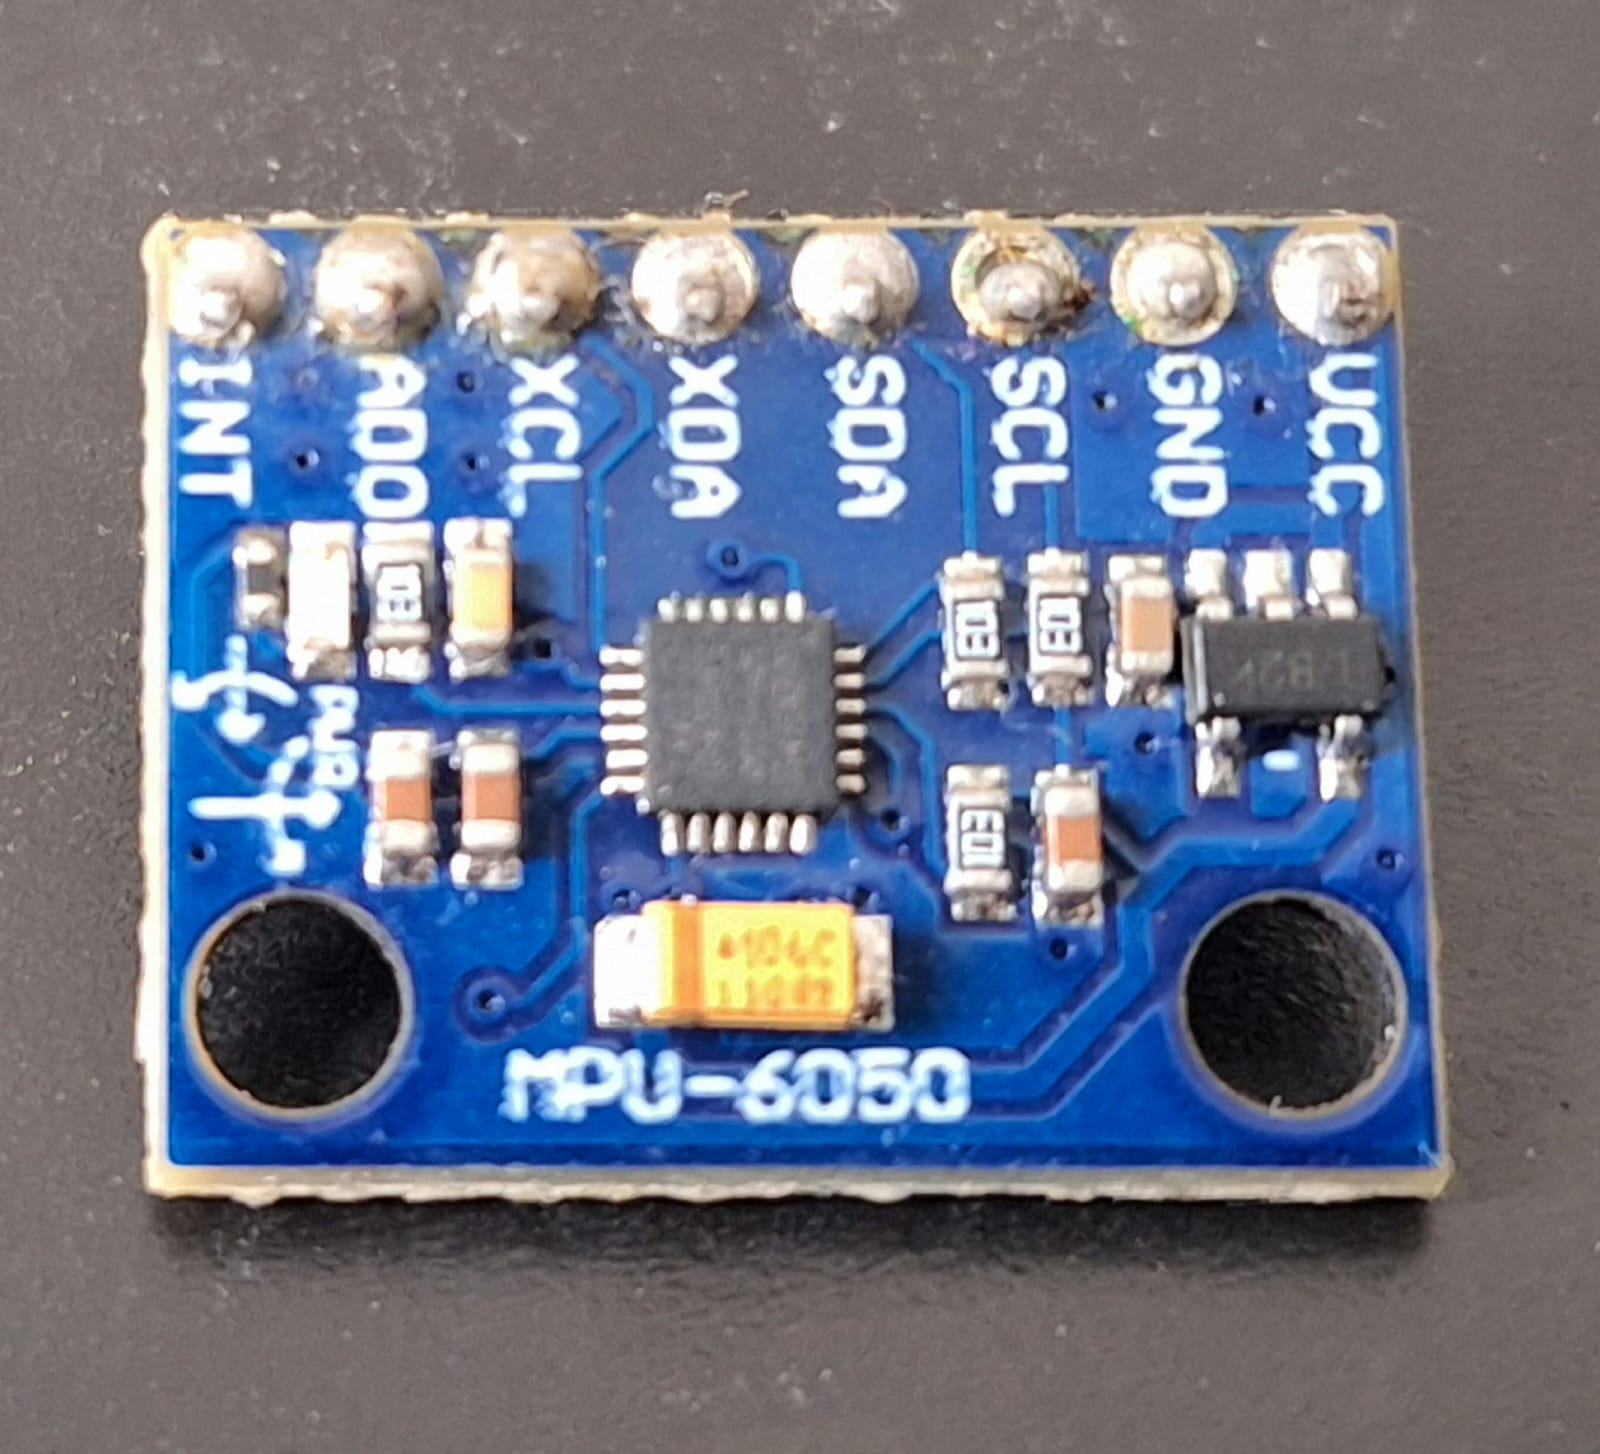
\includegraphics[height=4.1cm]{imagens/MPU6050.jpeg}}
                \label{fig:sensora}
            }\hfill
            \subfloat[MPU9250]{
                \frame{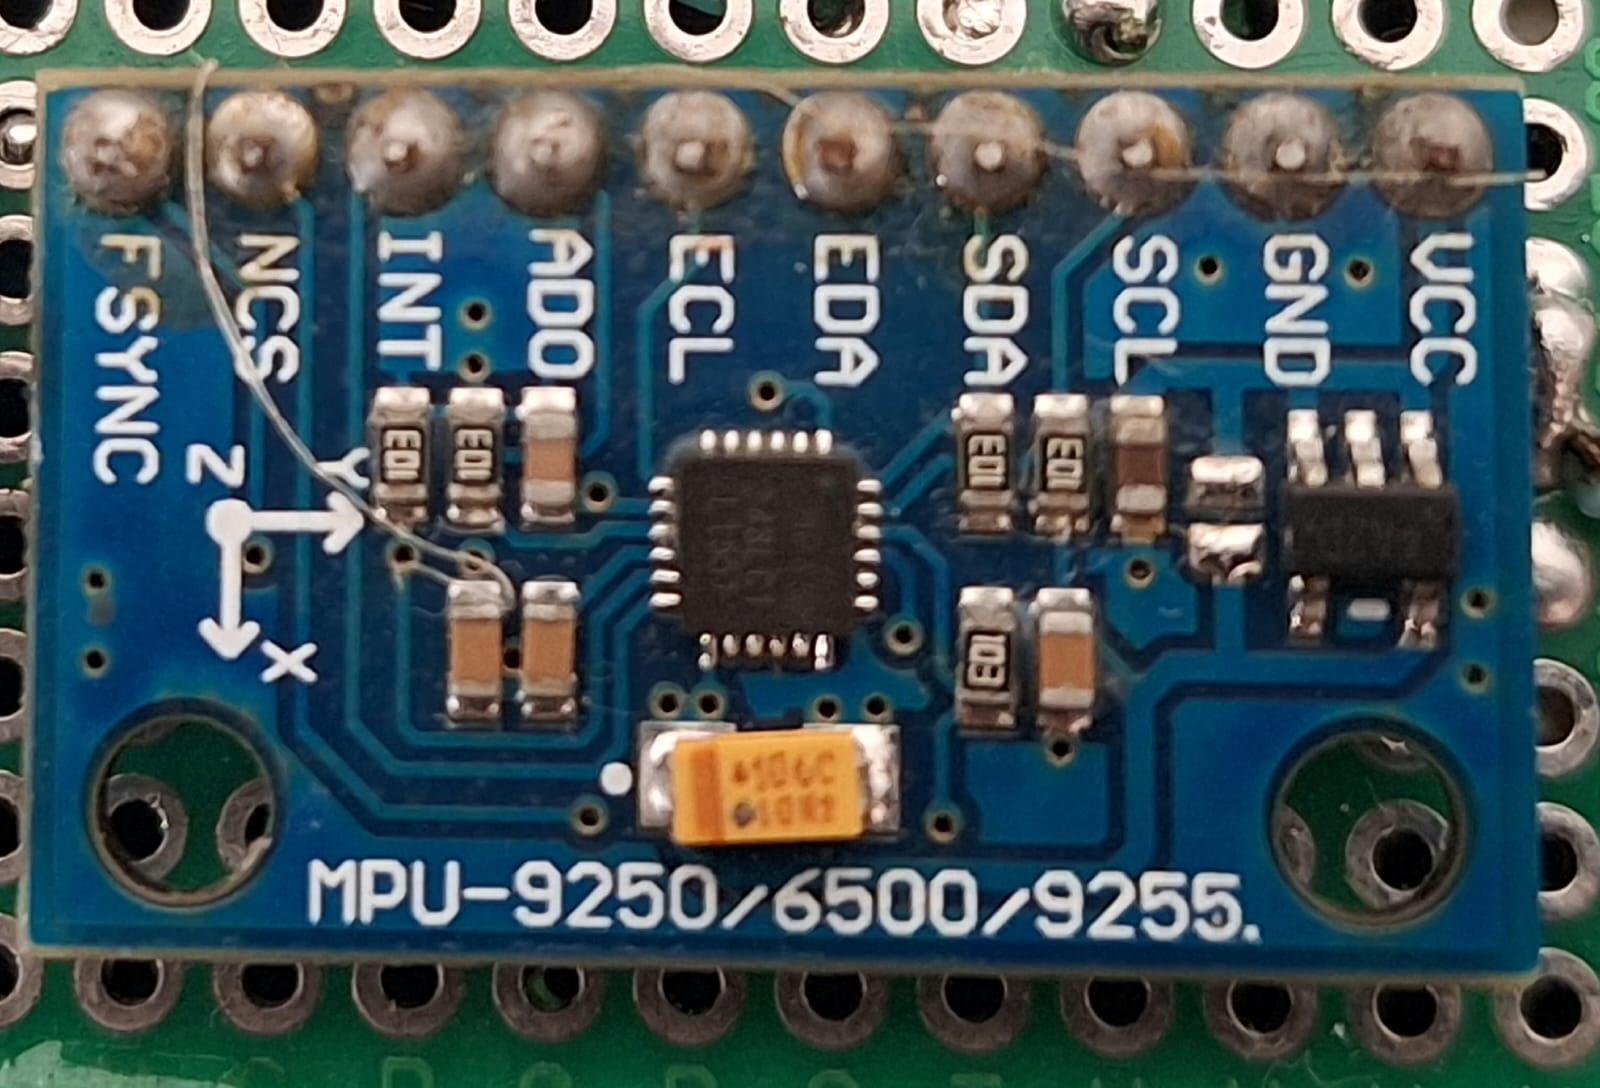
\includegraphics[height=4.1cm]{imagens/MPU9250.jpeg}}
                \label{fig:sensorb}
            }\hfill
            \subfloat[Kernel Sensor]{
                \frame{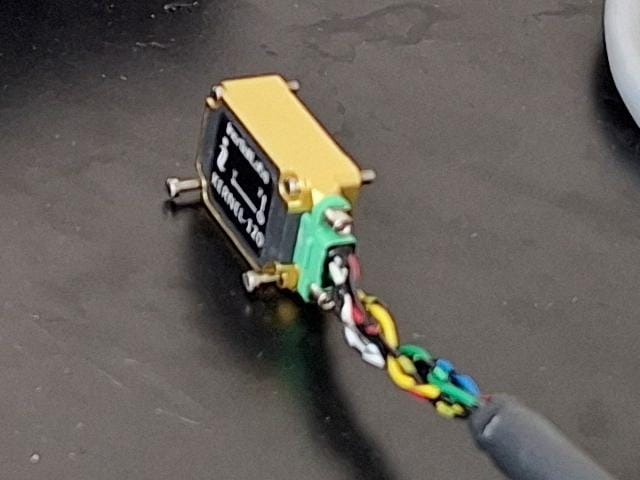
\includegraphics[height=4.1cm]{imagens/Kernel.jpeg}}  
                \label{fig:sensorc}
            }
            
            \textbf{Fonte:} Autor
            \label{fig:placeholder}
        \end{figure}

        O MPU6050, mostrado na Figura\autoref{fig:sensora}, combina um acelerômetro de três eixos e um giroscópio também de três eixos. Essa configuração de seis eixos, frequentemente chamada de 6DOF (graus de liberdade, em português), permite capturar movimentos de translação e rotação. Por essa razão, o componente é amplamente empregado em aplicações como robótica, drones e eletrônicos vestíveis para monitorar orientação, vibração e dinâmica angular (JIAN, 2016). Apesar do seu baixo custo e menor precisão, este sensor é benéfico ao projeto pois os algoritmos de fusão podem ser implementados de modo a compará-lo com sensores mais precisos, servindo de "gabarito"\ para validar a eficácia do filtro.

        Similar ao 6050, o MPU9250 (Figura\autoref{fig:sensorb}) também realiza a medição três eixos a partir do acelerômetro e giroscópio, mas também conta com um magnetômetro, que permite uma determinação de orientação mais completa e robusta, já que adiciona a capacidade de medir o campo magnético terrestre conforme mostrado no estudo de Komary (2022). Isso possibilita obter uma orientação absoluta em relação ao norte magnético, tornando-o superior para aplicações que exigem uma bússola eletrônica confiável, como sistemas de navegação e posicionamento.
    
        Já o Inertial Labs KERNEL (\autoref{fig:kernel2}) é uma IMU MEMS de classe industrial/tática com acelerômetros e giroscópios triaxiais de baixo ruído e alta repetibilidade pensadas para aplicações dinâmicas exigentes. Essa família opera com interface RS-422 (até 2 Mbit/s) e atualização interna de 2 kHz, mais do que suficiente para o escopo do projeto. Em síntese, o KERNEL serve como “padrão ouro” no conjunto, providenciando medições de alta fidelidade e temporização determinística para validar filtros e calibrar sensores de baixo custo como o MPU6050/9250 no mesmo experimento.

        \begin{figure}[H]
            \centering
            \caption{Sistema de Coordenadas do Sensor Kernel}
            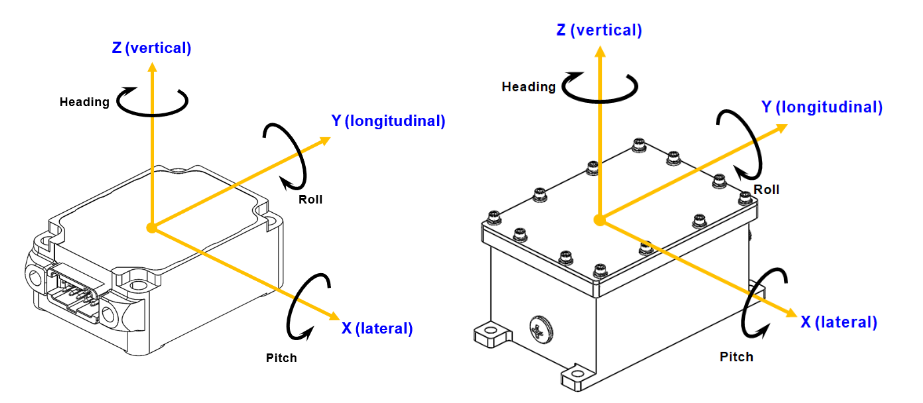
\includegraphics[width=0.9\linewidth]{imagens/kernel2.png}

            \textbf{Fonte:} \href{https://inertiallabs.com/}{Inertial Labs} 
            \label{fig:kernel2}
        \end{figure}
    
        Um ponto importante, descrito na documentação do Kernel, pode ser aplicado aos algoritmos atuais para aprimorar a calibração e a estabilização do sistema. Segundo o documento, recomenda-se que a unidade permaneça imóvel por até 30 segundos para uma estimativa mais precisa do erro sistemático (bias), embora exista a opção de inicialização em movimento, que acarreta perda de precisão dinâmica. A combinação desse procedimento com a lógica de Zero Velocity Update (ZUPT), técnica de atualização por velocidade zero, resulta em uma melhor orientação do sensor antes do início do regime contínuo de medição. A implementação dessa abordagem em sensores alternativos apresenta-se como uma solução viável para otimizar o processo de calibração.

    \subsection{Tabela Comparativa}
        Com base na seção anterior onde todos os sensores foram apresentados, uma tabela comparativa foi elaborada para que fique possível selecionar de forma objetiva o sensor adequado para o projeto, levando em conta a precisão, estabilidade e robustez.

        \begin{center}
            {\renewcommand{\arraystretch}{1.5}
            \begin{longtable}{|c|c|c|c|}
                \caption{Comparação de especificações (MPU6050, MPU9250 e KERNEL-110/120)} \label{tab:imus}\\
                \hline
                    \textbf{Especificação} & 
                    \textbf{MPU6050} & 
                    \textbf{MPU9250} & 
                    \textbf{KERNEL-110/120} \\
                \hline
                    \fcol{.22}{Densidade de ruído\\(gyro; accel)} &
                    \col{.26}{0{,}005 $^\circ$/s/$\sqrt{\text{Hz}}$; 400 $\mu$g/$\sqrt{\text{Hz}}$} &
                    \col{.26}{0{,}01 $^\circ$/s/$\sqrt{\text{Hz}}$; 300 $\mu$g/$\sqrt{\text{Hz}}$} &
                    \col{.26}{0{,}3 $^\circ$/h; 0{,}02 m/s$^{2}$/$\sqrt{\text{Hz}}$} \\
                \hline
                    \fcol{.22}{Estabilidade de \textit{bias} do giroscópio\\(@ 25$^\circ$C; variação c/ temperatura)} &
                    \col{.26}{$\pm$20 $^\circ$/s inicial; $\pm$20 $^\circ$/s c/ temp.} &
                    \col{.26}{$\pm$5 $^\circ$/s inicial; $\pm$30 $^\circ$/s c/ temp.} &
                    \col{.26}{2 $^\circ$/h (in-run); 72 $^\circ$/h} \\
                \hline
                    \fcol{.22}{Não-linearidade\\(\% do intervalo de medição)} &
                    \col{.26}{0{,}2 \% FS} &
                    \col{.26}{0{,}1 \% FS} &
                    \col{.26}{0{,}035 \% FS (350 ppm)} \\
                \hline
                    \fcol{.22}{Largura de banda\\(-3 dB cutoff)} &
                    \col{.26}{\textasciitilde256 Hz (prog.\ DLPF)} &
                    \col{.26}{\textasciitilde250 Hz (prog.\ DLPF)} &
                    \col{.26}{260 Hz} \\
                \hline
                    \fcol{.22}{Taxa máxima de atualização\\\textit{Output Data Rate}} &
                    \col{.26}{Gyro 8 kHz; Accel 1 kHz} &
                    \col{.26}{Gyro 8 kHz; Accel 4 kHz} &
                    \col{.26}{Gyro 2 kHz; Accel 2 kHz} \\
                \hline
                    \fcol{.22}{Fonte} &
                    \col{.26}{\href{https://www.alldatasheet.com/datasheet-pdf/pdf/1132807/TDK/MPU-6050.html}{\textbf{ALL DATASHEET}}} &
                    \col{.26}{\href{https://invensense.tdk.com/wp-content/uploads/2015/02/PS-MPU-9250A-01-v1.1.pdf}{\textbf{Iven Sense}}} &
                    \col{.26}{\href{https://inertiallabs.com/}{\textbf{Inertial Labs}}} \\
                \hline
            \end{longtable}
            }
            \textbf{Fonte:} Autor
        \end{center}

        De acordo com a tabela, torna-se evidente, portanto, que para maior precisão/estabilidade, o Inertial Labs KERNEL-110/120 é superior, já que estabilidade de bias do giroscópio de ~2 °/h (in-run), que é ordens de grandeza melhor que os ±5–20 °/s dos MPU6050/9250, além de não-linearidade menor (0,035\% FS vs 0,1–0,2\% FS); como a deriva de bias e a linearidade dominam o erro acumulado em navegação e medição de atitude, esse desempenho implica deriva muito mais baixa e repetibilidade maior ao longo do tempo e da temperatura, mesmo com largura de banda similar (~260 Hz) e apesar de um ODR menor.
        
    \newpage
    \subsection{Prototipação das Placas de Circuito Impresso}  
        A placa desenvolvida exclusivamente para fins de testes, representada nas figuras \ref{fig:pcbtestea} e \ref{fig:pcbtesteb}, foi produzida conforme as esquematizações documentadas na macroentrega anterior. Sua, função principal é a integração a diversos circuitos, permitindo a validação do primeiro protótipo por meio de testes individuais de componentes. Foram realizadas verificações nos Circuitos Integrados de comunicação, na alimentação dos sensores, na análise de capacitores e na estabilidade com o microcontrolador principal. Também foi monitorada e avaliada a proteção do circuito contra flutuações de tensão e corrente.

        \vspace{-.1cm}
        \begin{figure}[H]
            \centering
            \caption{Prototipagem Placas de Circuito Impresso}
      
            \subfloat[]{
                \frame{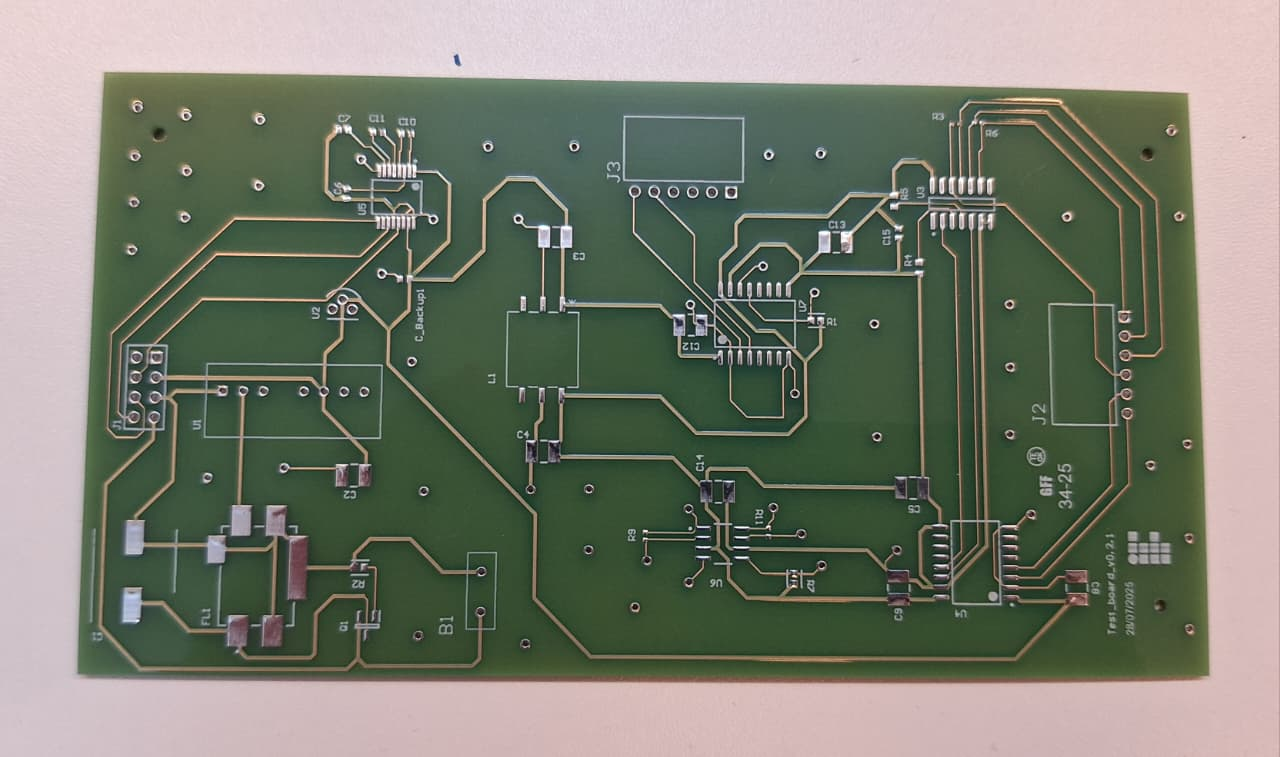
\includegraphics[height=4.9cm]{imagens/raw_pcb_1.jpeg}}
                \label{fig:pcbtestea}
            }
            \hfill
            \subfloat[]{
                \frame{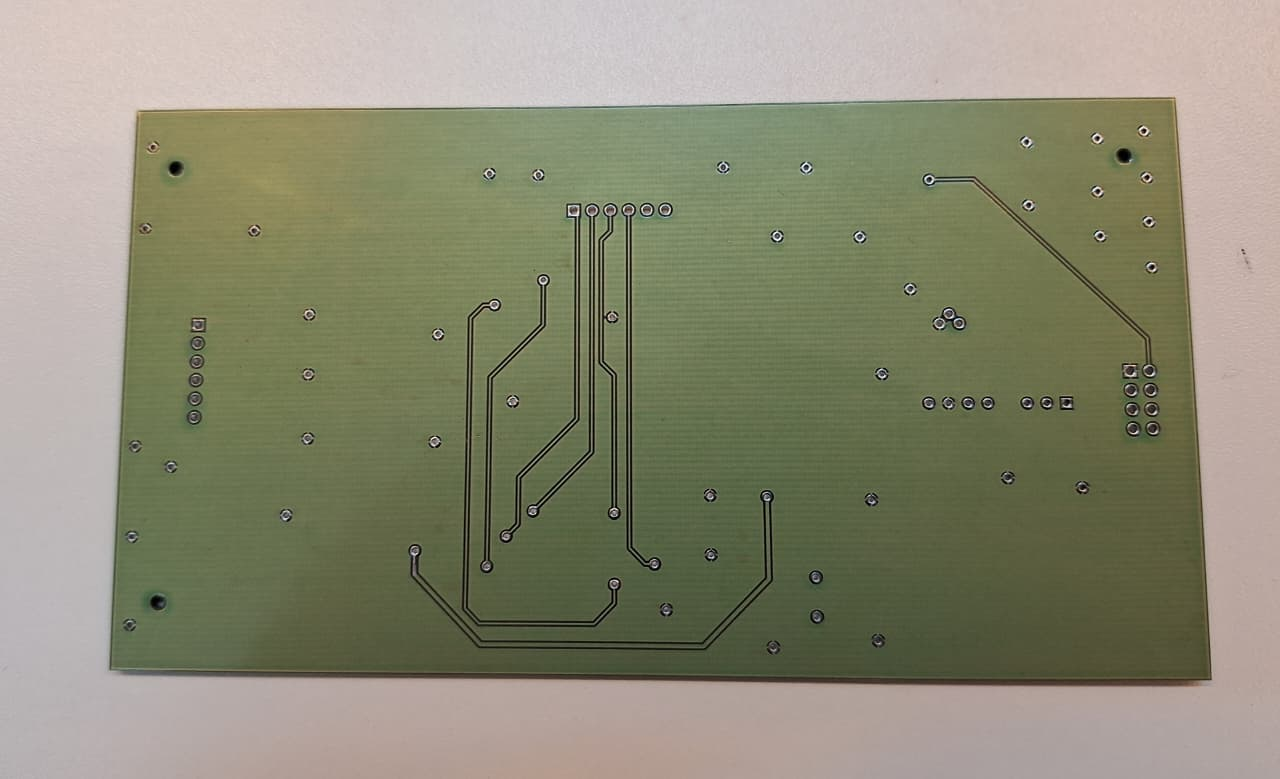
\includegraphics[height=4.9cm]{imagens/raw_pcb_2.jpeg}}
                \label{fig:pcbtesteb}
            }
        
            \textbf{Fonte:} Autor
            \label{fig:placas}
        \end{figure}

    A necessidade de uma placa dedicada exclusivamente aos testes surgiu da prática anterior de verificar componentes, como os módulos de comunicação RS-232 e RS-422, bem como os circuitos de alimentação, de maneira isolada e sem integração entre si. A nova placa oferece a vantagem de permitir a avaliação individual e simultânea de múltiplos componentes em um único circuito dedicado à validação, solucionando problemas comuns em protoboards, como falhas de conexão, excesso de fios e a falta de clareza visual, que são essenciais para uma depuração eficiente do sistema. Dessa forma, os testes foram conduzidos conforme o planejado, possibilitando a seleção e a verificação adequada dos melhores módulos para, então, proceder com o desenvolvimento da versão final do projeto.

    Além disso, a placa de testes viabilizou a validação de diversos circuitos integrados na versão SMD (Dispositivo de Montagem em Superfície, do inglês Surface Mount Device), tecnologia que permite a fabricação de equipamentos eletrônicos significativamente mais compactos, leves e eficientes, como os utilizados em smartphones e notebooks. Por outro lado, os componentes PTH (Through-Hole Technology), de montagem convencional, possuem dimensões maiores, demandam mais espaço físico e estão mais sujeitos a falhas, como soldas frágeis ou descolamento acidental. Dessa forma, a adoção da tecnologia SMD, validada por meio da placa, trouxe ganhos adicionais, como a expressiva redução de custos e o aumento geral da confiabilidade do produto final.


    \subsection{Montagem das Placas}
        Ao final dos testes mencionados, todos os componentes de interesse foram soldados na placa, resultando nas figuras \ref{fig:placas/a} e \ref{fig:placas/b}. A validação dos componentes mostrou-se conforme o esperado e todos apresentaram bom desempenho o que permitiu a elaboração de uma placa final destinada a testes de campo.
        
        \begin{figure}[H]
            \centering
            \caption{Montagem das Placas de Circuito Impresso}
            
            \subfloat[]{
                \frame{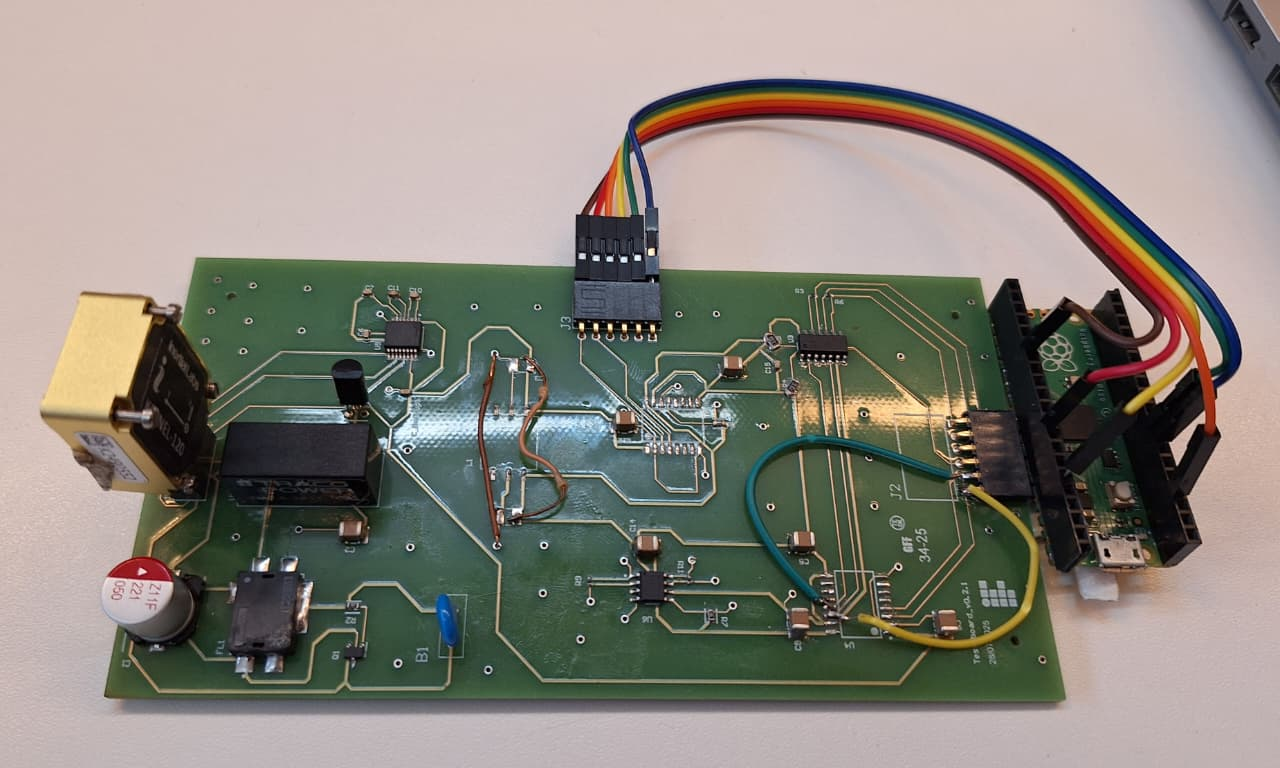
\includegraphics[height=5.5cm]{imagens/pcb_1.jpeg}}
                \label{fig:placas/a}
            }
            \hfill
            \subfloat[]{
                \frame{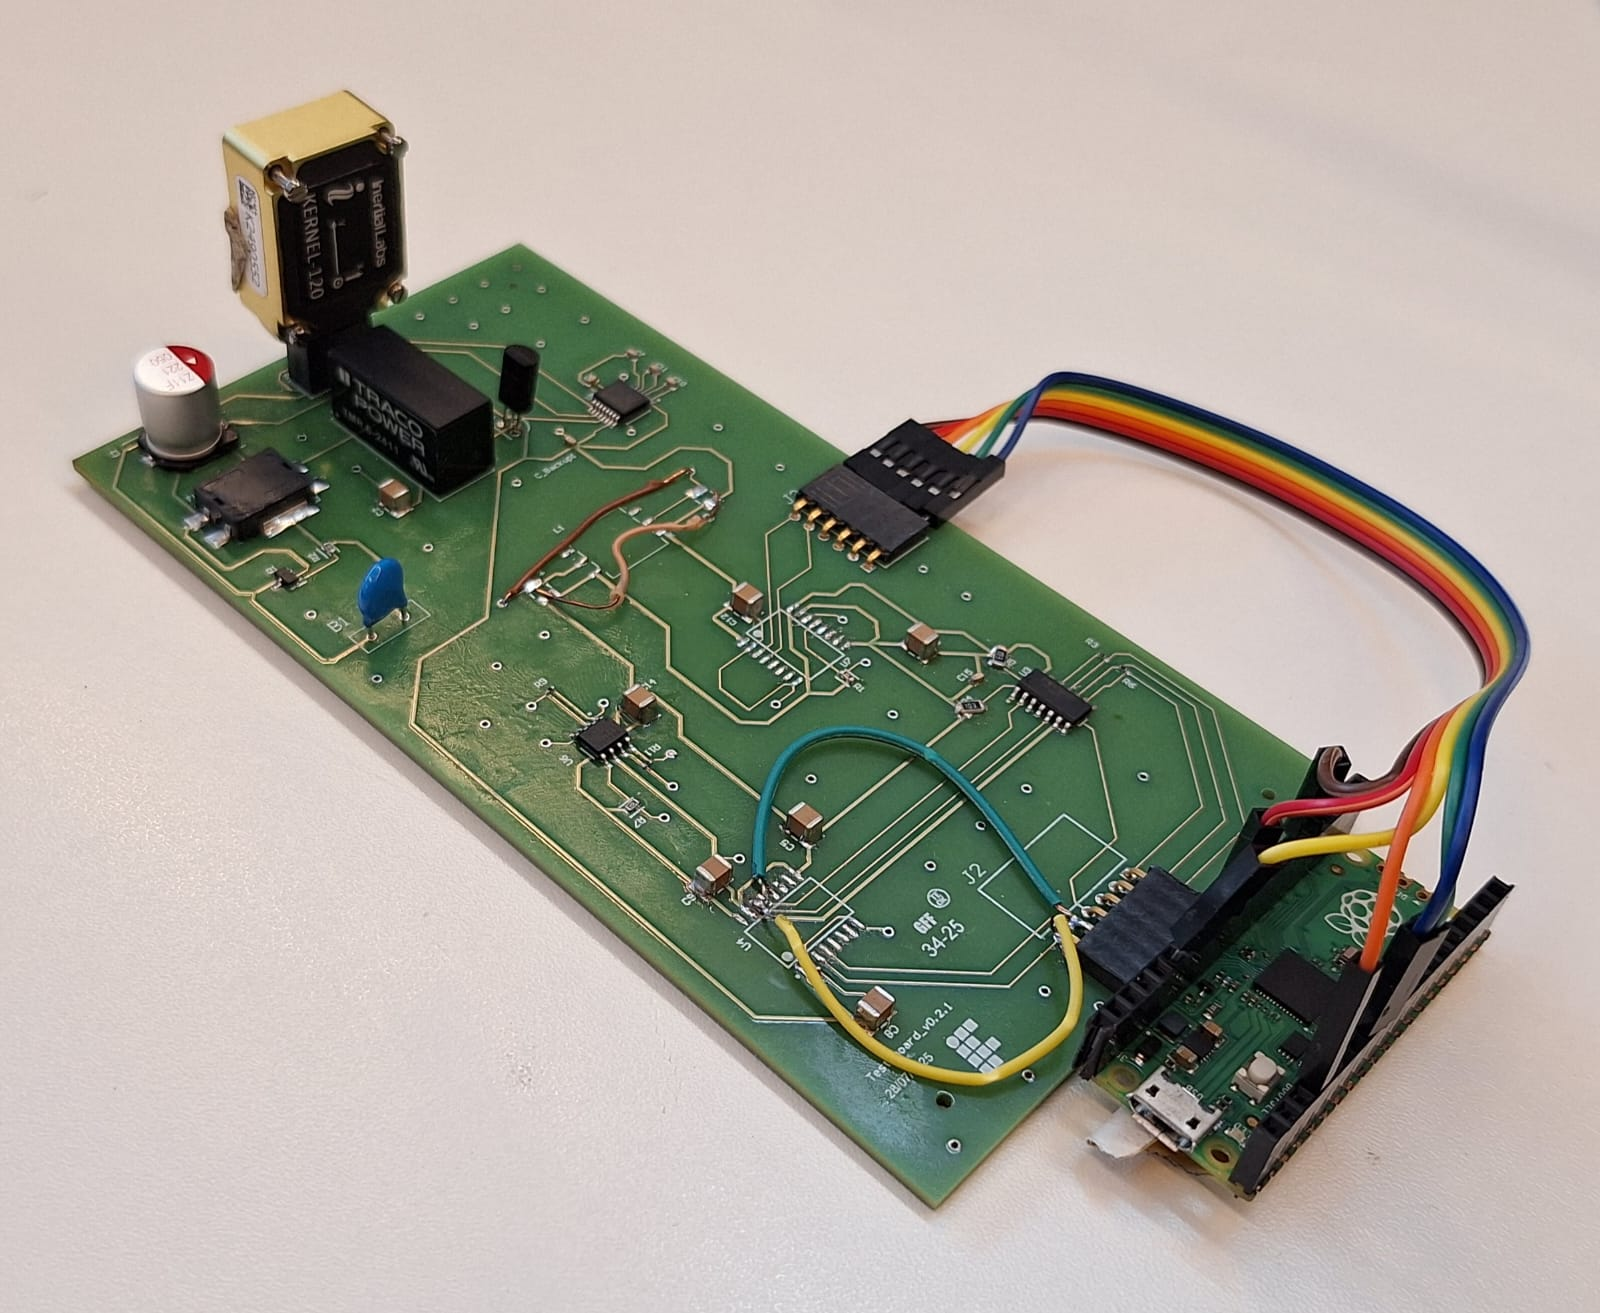
\includegraphics[height=5.5cm]{imagens/pcb_2.jpeg}}
                \label{fig:placas/b}
            }
        
            \textbf{Fonte:} Autor
            \label{fig:placas}
        \end{figure}

        O sensor Kernel foi testado em conjunto com a placa dedicada, conforme ilustrado na Figura\autoref{fig:placas/b}, interligado ao módulo de comunicação RS-422. Essa configuração permitiu validar a funcionalidade do sensor, que realizou com sucesso a transmissão e recepção de dados por meio do referido protocolo. Além dos testes de comunicação, foram realizados ensaios elétricos para verificar o comportamento do componente sob variações de tensão e corrente. Os resultados demonstraram que o sensor apresenta resistência a picos de energia, graças a um circuito de proteção integrado, o que elimina a necessidade de preocupações adicionais com esses aspectos e permite que a equipe foque diretamente na etapa de implementação técnica.

        O circuito foi alimentado com uma tensão variável entre 16 e 29 volts para verificar o correto funcionamento da fonte chaveada e avaliar o comportamento dos componentes eletrônicos dentro da faixa de operação padrão definida para o projeto. Os testes demonstraram que todos os elementos responderam adequadamente, sem apresentar falhas ou alterações de desempenho, confirmando a estabilidade do sistema tanto na comunicação quanto nos parâmetros elétricos essenciais.


    \subsection{Compartimento Dedicado}
        O compartimento destinado às placas, as quais o desenho técnico se encontram nas figuras a seguir, foi projetado para acomodar os sensores em uma estrutura fechada que confere resistência e proteção aos componentes em ambientes adversos, viabilizando a realização de testes em campo. Dessa forma, o protótipo dentro da embalagem possibilita a verificação dos códigos e o acompanhamento das variáveis de modo mais eficiente, além de contribuir para um aprimoramento na calibração dos sensores.

        \begin{figure}[H]
            \centering
            \caption{Desenhos Técnicos do Compartimento}

            \subfloat[Tampa Superior]{
                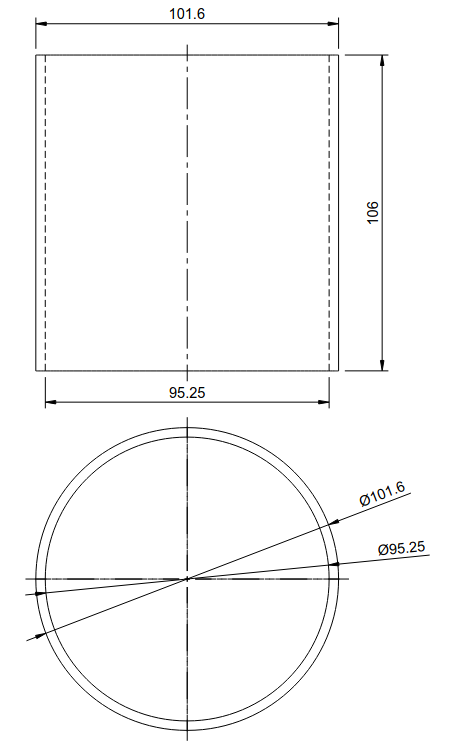
\includegraphics[height=7cm]{imagens/desenhoA.png}
            }
            \hfill
            \subfloat[Tampa Inferior]{
                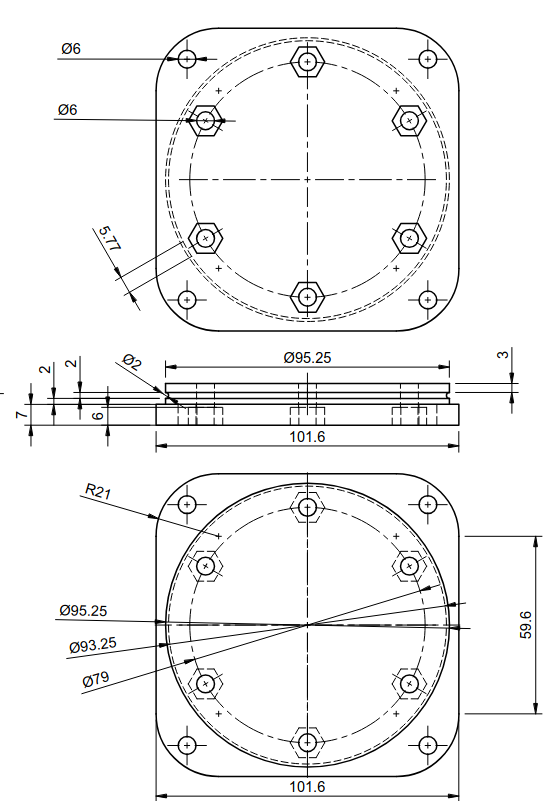
\includegraphics[height=7cm]{imagens/desenhoB.png}
            }
            \hfill
            \subfloat[Cilindro]{
                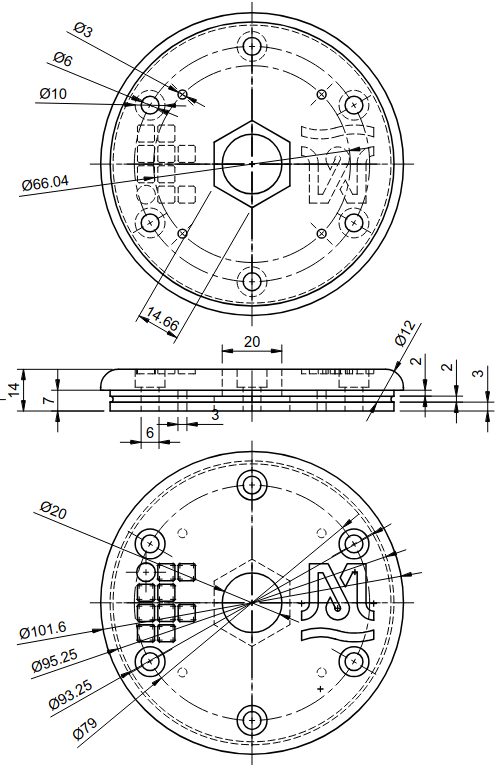
\includegraphics[height=7cm]{imagens/desenhoC.png}
            }

            \textbf{Fonte:} Autor
            \label{fig:placeholder}
        \end{figure}
        
        Os desenhos técnicos podem ser encontrados no \textbf{Anexo I}. O compartimento descrito foi produzido por impressão 3D e pode ser observado nas Figuras \ref{fig:impA} e \ref{fig:impB}.

        \begin{figure}[H]
            \centering
            \caption{Compartimento do Circuito Feito em Impressora 3D}

            \subfloat[]{
                \frame{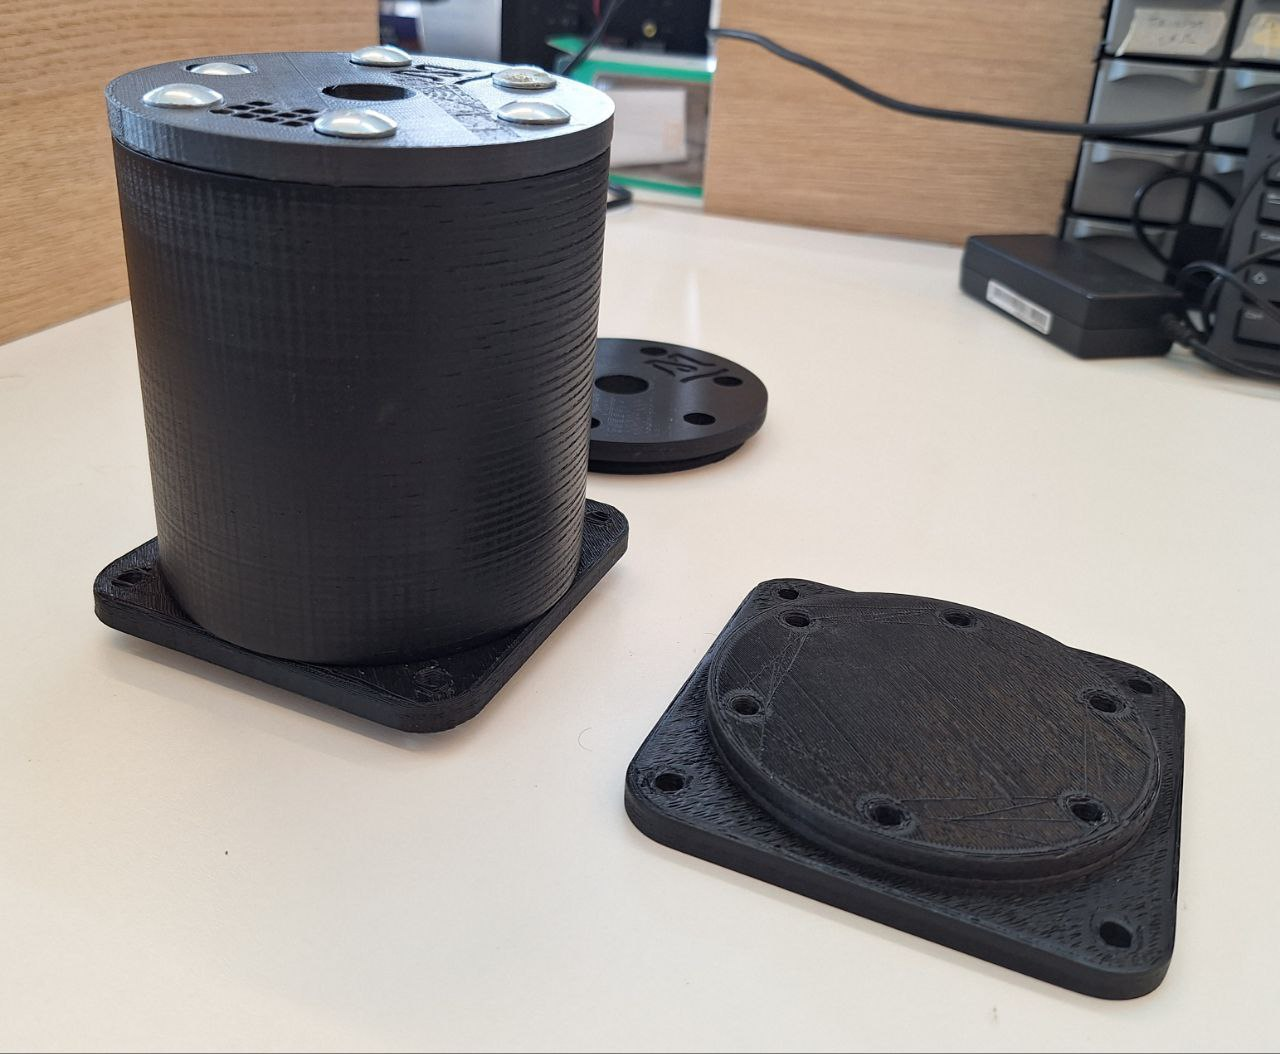
\includegraphics[height=7cm]{imagens/embalagem01.jpeg}}
                \label{fig:impA}
            }
            \hspace{.5cm}
            \subfloat[]{
                \frame{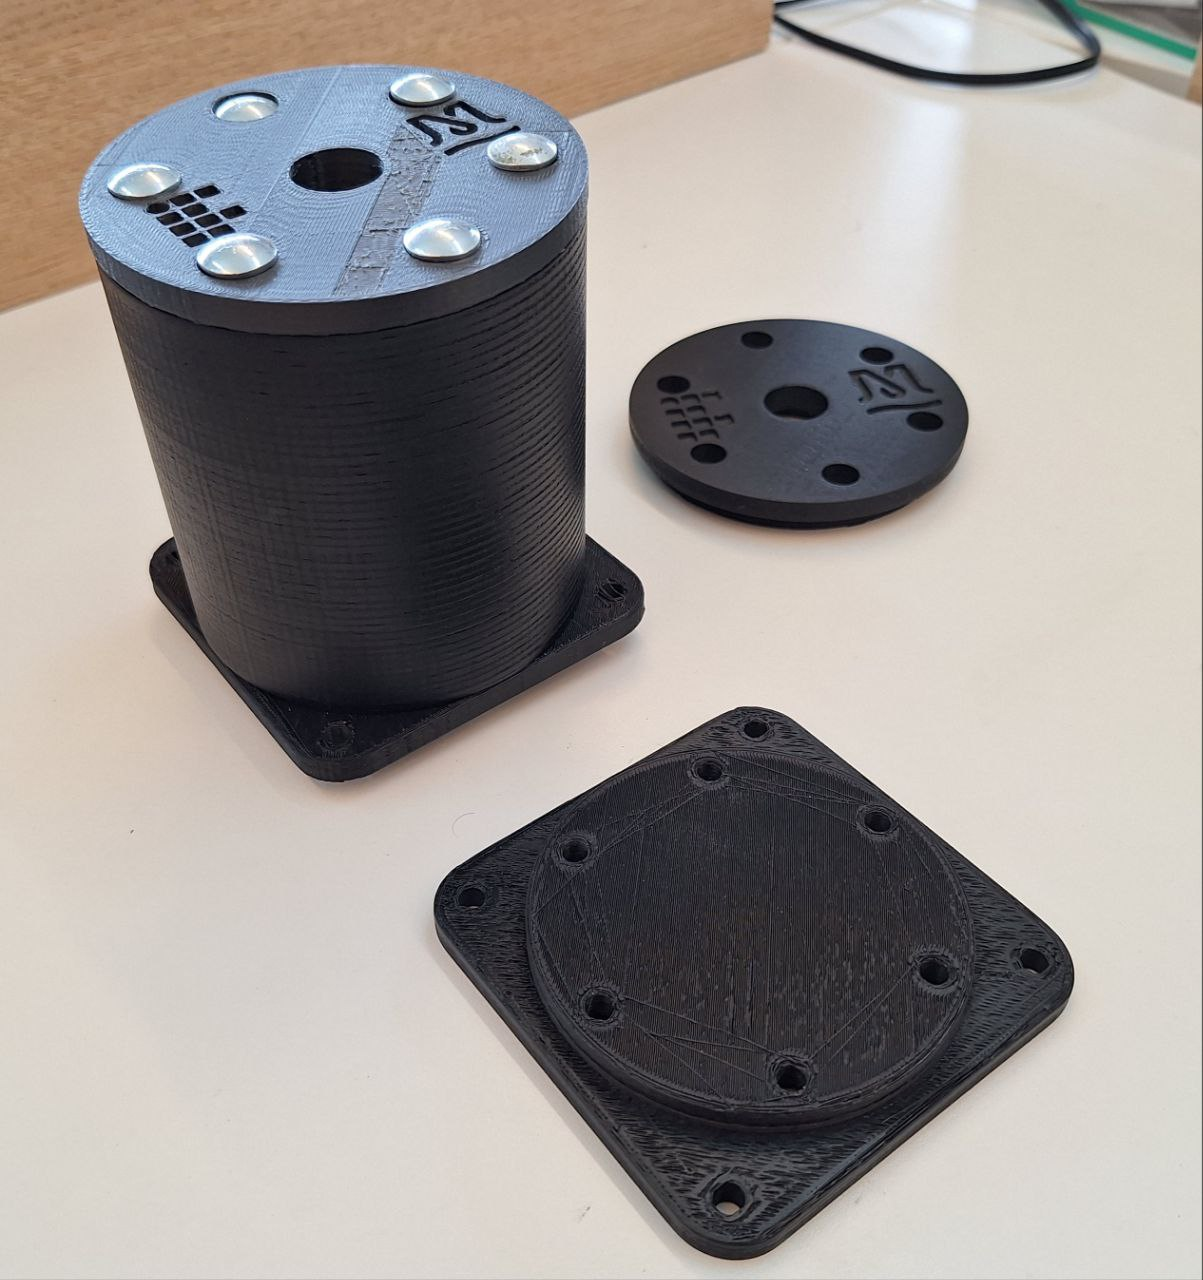
\includegraphics[height=7cm]{imagens/embalagem02.jpeg}}
                \label{fig:impB}
            }

            \textbf{Fonte:} Autor
            \label{fig:placeholder}
        \end{figure}


    \subsection{Placa do Primeiro Protótipo}
        A partir da validação dos componentes na placa de testes, a equipe prosseguiu para o desenvolvimento da placa definitiva do primeiro protótipo, mostrado na Figura\autoref{fig:placanova}. Esta placa integra o sensor principal, Kernel Sensor, e o microcontrolador ESP32, que funciona como a unidade central do sistema. A placa foi projetada para permitir a comunicação e o envio de dados para um dispositivo externo por meio do protocolo RS232. Com este protótipo em mãos, será possível realizar testes mais precisos e abrangentes, tanto em laboratório quanto em campo.
        \vspace{0.3cm}
        
        \begin{figure}[H]
            \centering
            \caption{Esquematização das PCBs do Primeiro Protótipo}
             
            \subfloat[]{
                \frame{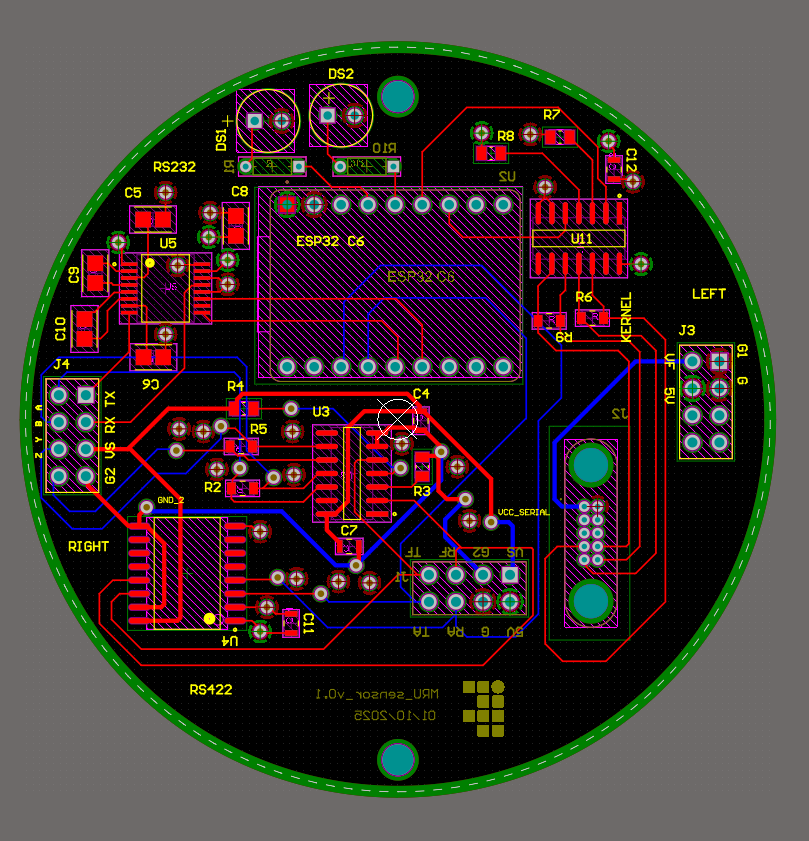
\includegraphics[height=8cm]{imagens/pcb_atilum_1.png}}
            }\hfill
            \subfloat[]{
                \frame{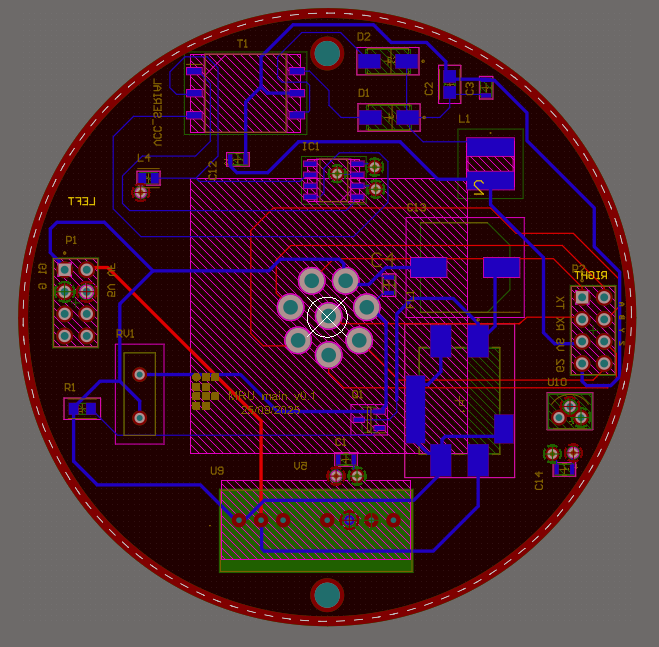
\includegraphics[height=8cm]{imagens/pcb_atilum_2.png}}
            }

            \textbf{Fonte:} Autor
            \label{fig:placanova}
        \end{figure}

        A principal alteração incorporada na versão preliminar da placa consiste na substituição do microcontrolador principal pelo modelo ESP32-S3 Mini, que mantém a mesma capacidade de processamento de 240 MHz, memória flash de 4 MB e PSRAM de 2 MB, porém em dimensões reduzidas de 1,54 cm por 2,05 cm. Essa significativa redução física permite uma maior compactação do circuito, oferecendo mais flexibilidade para o design do invólucro e do compartimento dos componentes. Adicionalmente, o microcontrolador selecionado apresenta melhor desempenho térmico, gerando menos calor durante operação, e facilita futuras integrações com elementos de dissipação, quando necessário. A \autoref{fig:spressif} mostra as dimensões do novo microcontrolador.

        \begin{figure}[H]
            \centering
            \caption{Dimensões do ESP32-Mini}
            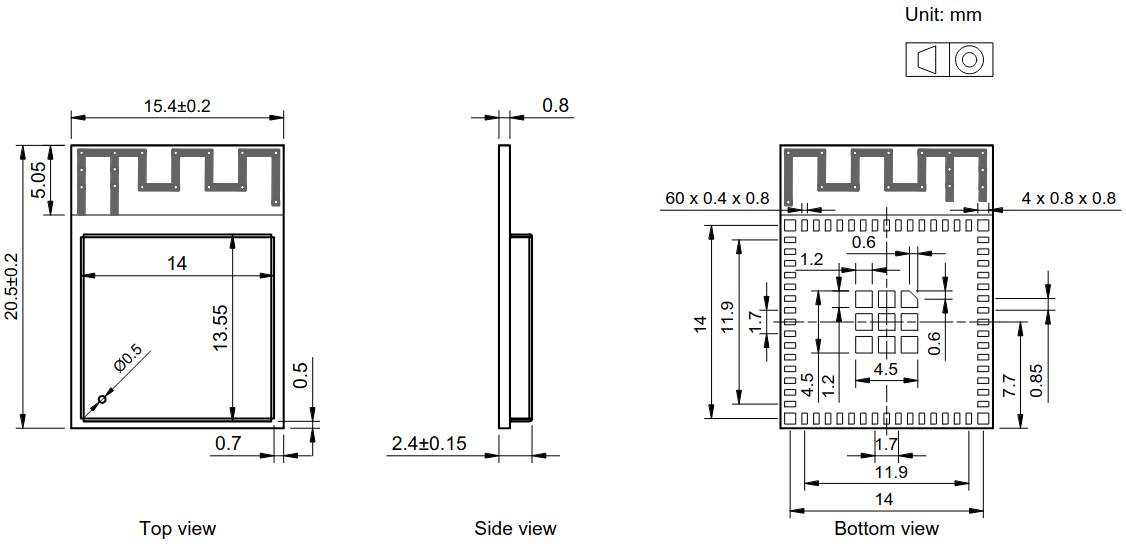
\includegraphics[width=\linewidth]{imagens/miniiii.png}

            \textbf{Fonte}: Espressif
            \label{fig:spressif}
        \end{figure}

        Com base no definido, a placa final foi esquematizada em um modelo tridimensional por meio do software próprio para desenvolvimento de PCBs (Printed Circuit Boards), conforme apresentado na figura seguinte, na qual todos os componentes estão dispostos de forma visível e organizada, permitindo uma compreensão clara de sua configuração física e viabilizando ajustes precisos no circuito antes da fabricação.

        \begin{figure}[H]
            \centering
            \caption{Visualização 3D das PCBs}
             
            \subfloat[]{
                \frame{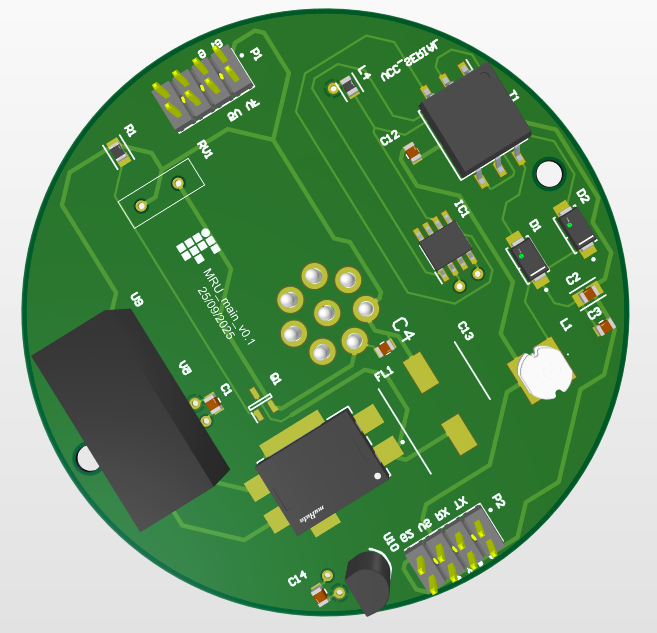
\includegraphics[height=4.8cm]{imagens/pcb_3d_1.png}}
            }\hfill
            \subfloat[]{
                \frame{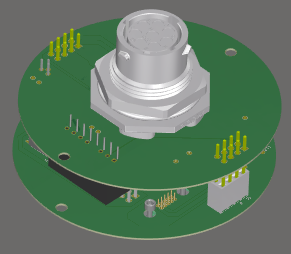
\includegraphics[height=4.8cm]{imagens/pcb_3d_2.png}}
            }\hfill
             \subfloat[]{
                \frame{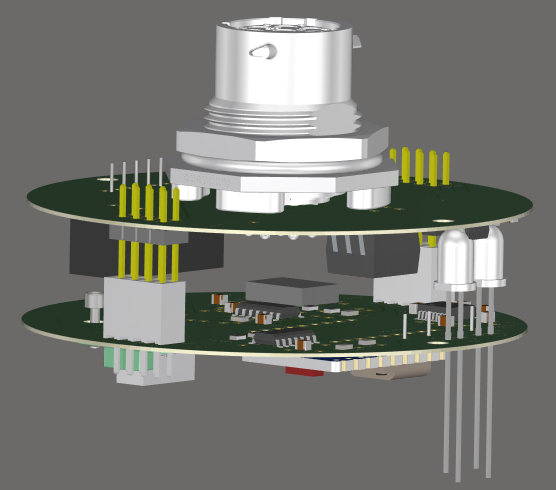
\includegraphics[height=4.8cm]{imagens/pcb_3d_3.png}}
            }

            \textbf{Fonte:} Autor
            \label{fig:placeholder}
        \end{figure}

        
    \newpage
    \subsection{Euroware do DRMM (fusão e filtros)}
        Com o objetivo de realizar um teste preliminar do sistema antes da chegada dos componentes definitivos, como as placas de circuito impresso e a estrutura do hexapod, um protótipo simplificado foi construído sobre uma placa de fenolite, onde os terminais do microcontrolador Raspberry Pi e dos sensores foram soldados, conforme a \autoref{fig:servo}. Essa configuração permitiu avaliar a medição de aceleração e inclinação, monitorando todos os sensores em um mesmo eixo durante movimentos específicos. 

        \begin{figure}[H]
            \centering
            \caption{Protótipo de Monitoramento a Partir de Servo Motor}
            \frame{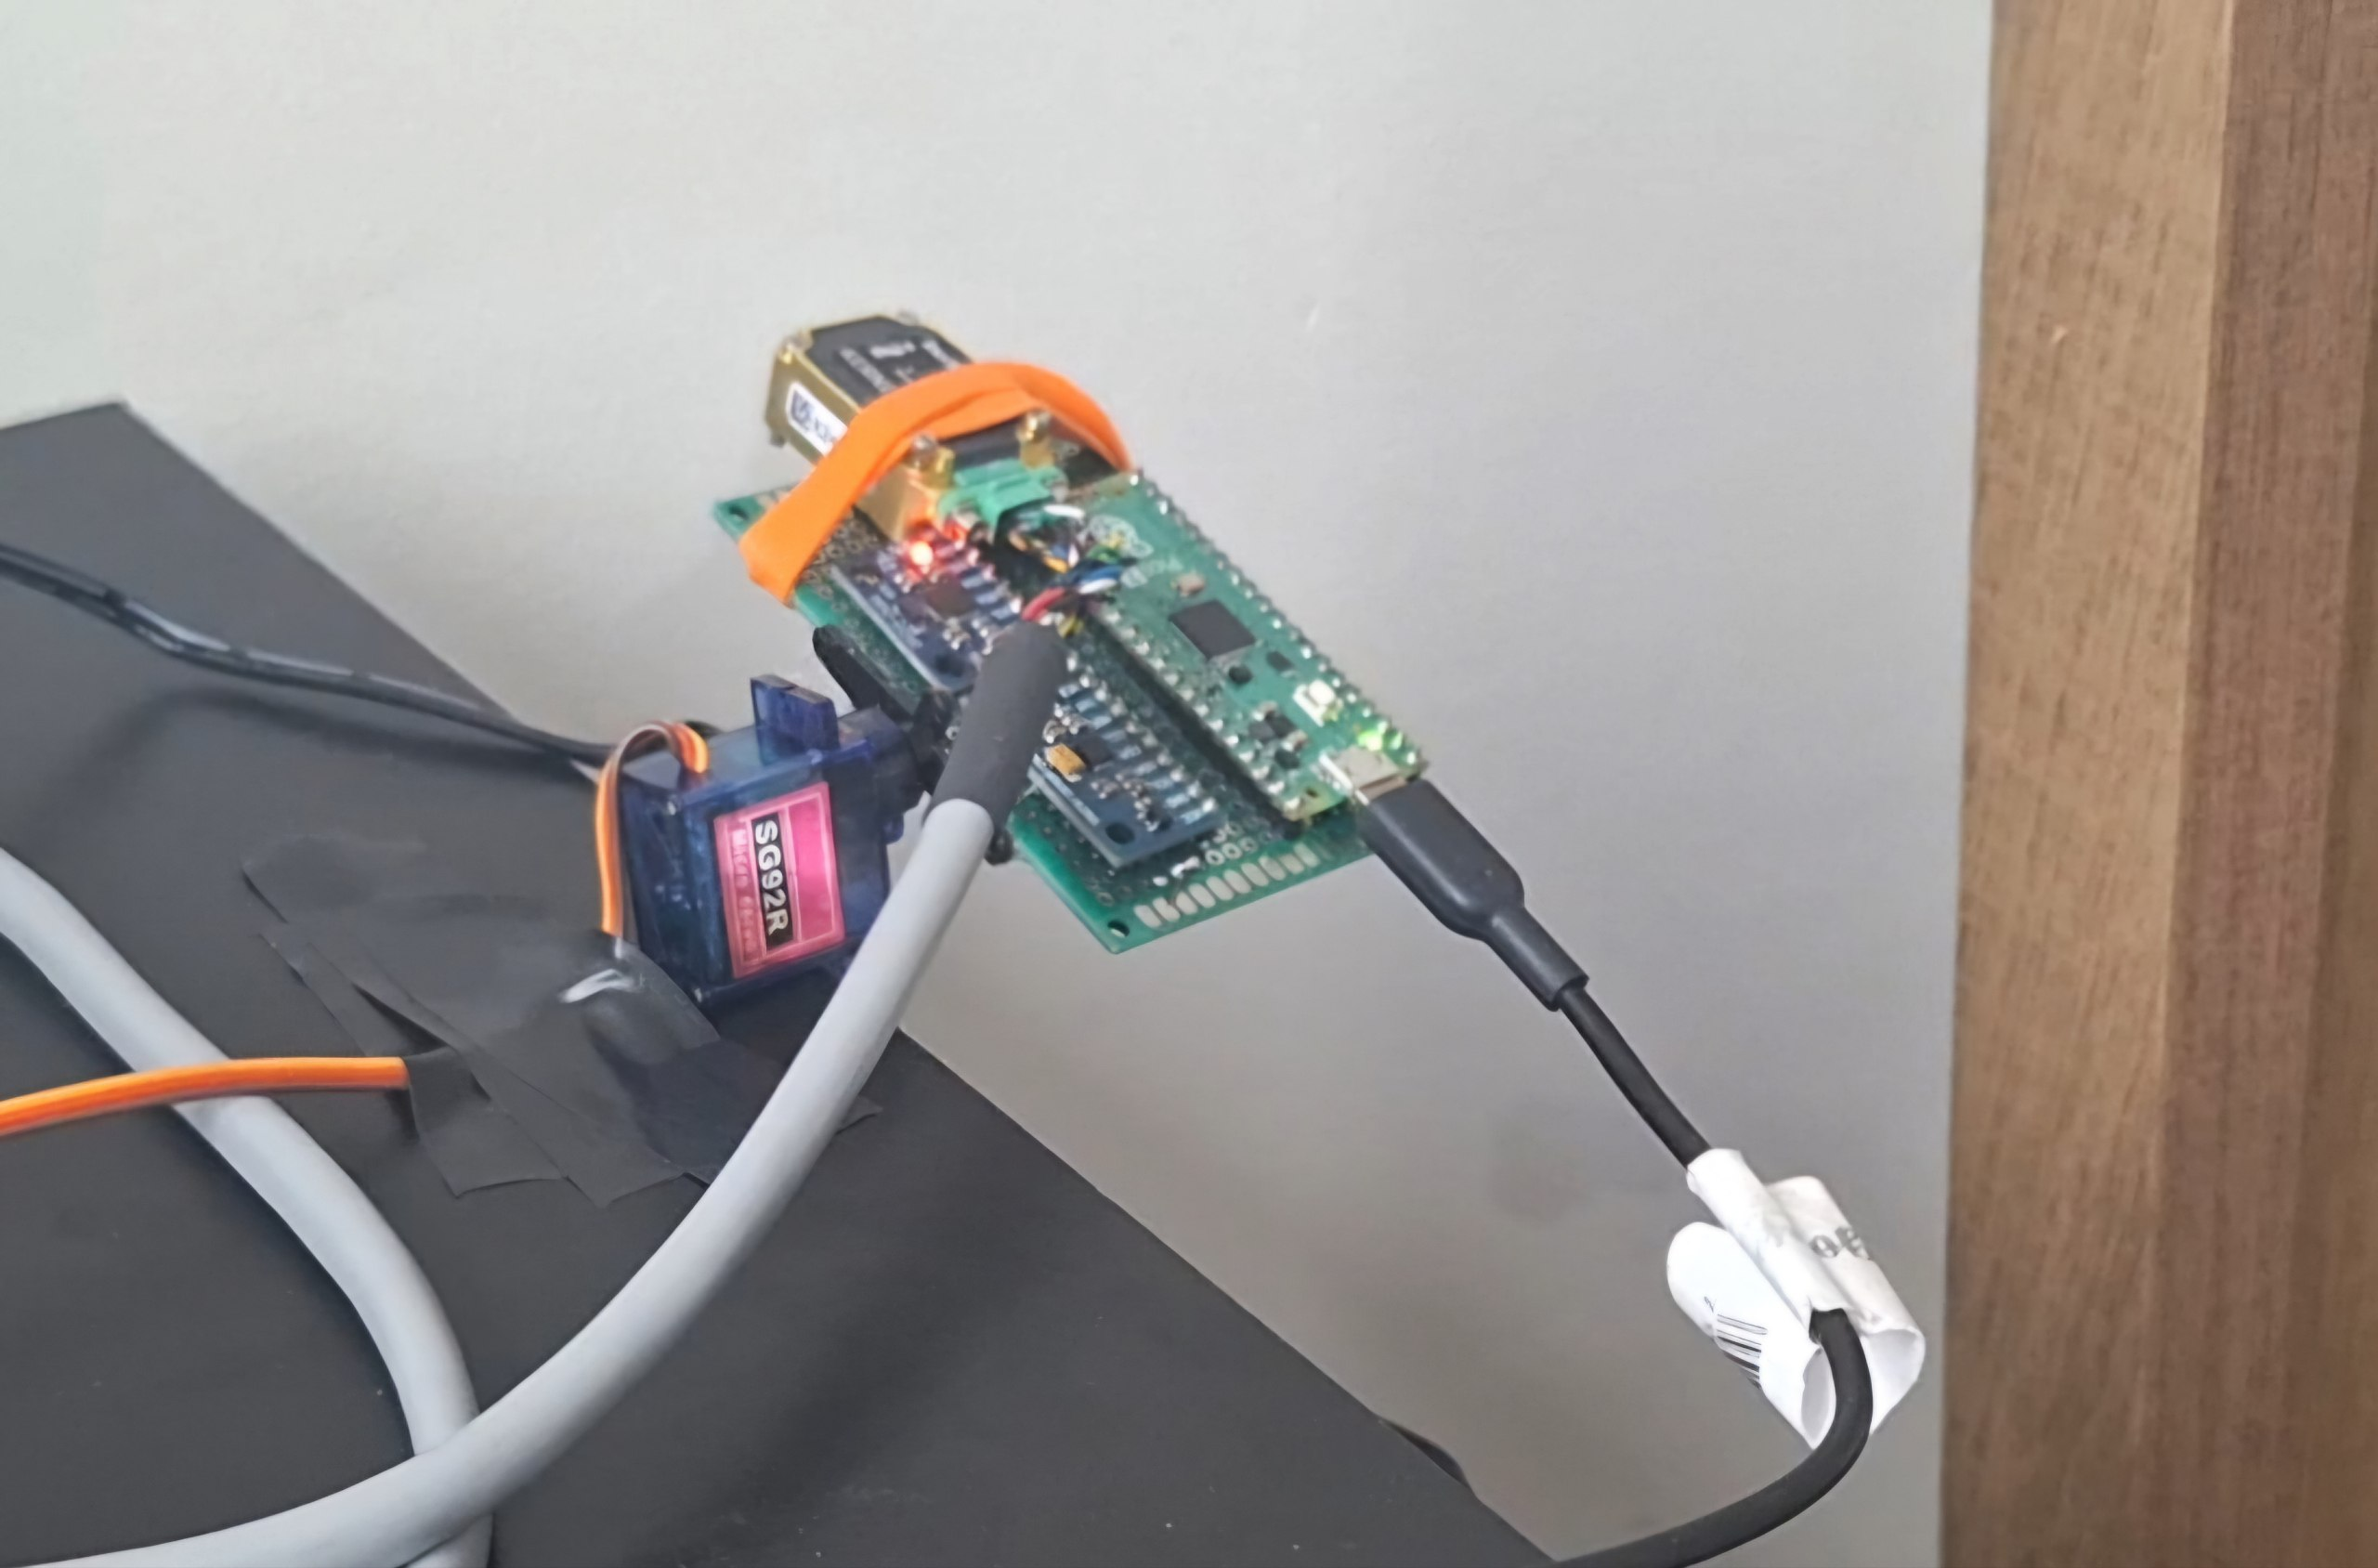
\includegraphics[width=.75\linewidth]{imagens/servo.jpg}}

            \textbf{Fonte:} Autor
            \label{fig:servo}
        \end{figure} 

        O acionamento foi feito por um servo motor de 5V controlado por um módulo Arduino UNO de maneira isolada, programado para executar rotações personalizadas de modo aleatório, a fim de identificar a presença de ruído e outliers nos dados. Embora a precisão obtida não seja elevada e sofra interferência de vibrações do motor, o método mostrou-se válido como ponto de partida para analisar o comportamento dos sensores.  No entanto, variações feitas de forma manual também foram realizadas de modo a verificar o impacto da vibração no sistema.

        O principal objetivo da abordagem descrita é comparar o desempenho de sensores do tipo MPU, de baixo custo e menor precisão, com o sensor Kernel, um dispositivo reconhecido por sua maior robustez e exatidão. A proposta é verificar se a aplicação de algoritmos de fusão e filtros digitais pode aprimorar o comportamento dos sensores menos precisos, atenuando o ruído de medição e validando o potencial de complementar o sensor de referência, e ser usado como um apoio em produção junto ao sensor principal.
        
        \newpage
        \subsubsection{Comparação em Modo Bruto}
            O estudo se inicia com a comparação dos sensores por meio de dados brutos, sem a utilização de filtros ou algoritmos de fusão, de modo a verificar o comportamento "padrão"\ dos componentes. Assim sendo, a comparação descrita foi feita utilizando-se o MPU0250, com o sensor Kernel (com filtros embutidos do próprio sensor). A \autoref{fig:raw} exibe a análise comparativa das variáveis de aceleração e angulação nos três eixos cartesianos. A análise do gráfico demonstra que, embora exista uma alta similaridade entre os sensores, uma simples inspeção visual permite identificar que os MPUs apresentam um nível de ruído mais elevado no sistema, exibindo flutuações e picos abruptos durante movimentos contínuos – comportamento que é corretamente capturado pelo sensor Kernel.
            
            \begin{figure}[H]
                \centering
                \caption{Comparação dos Sensores em Dados Brutos}
                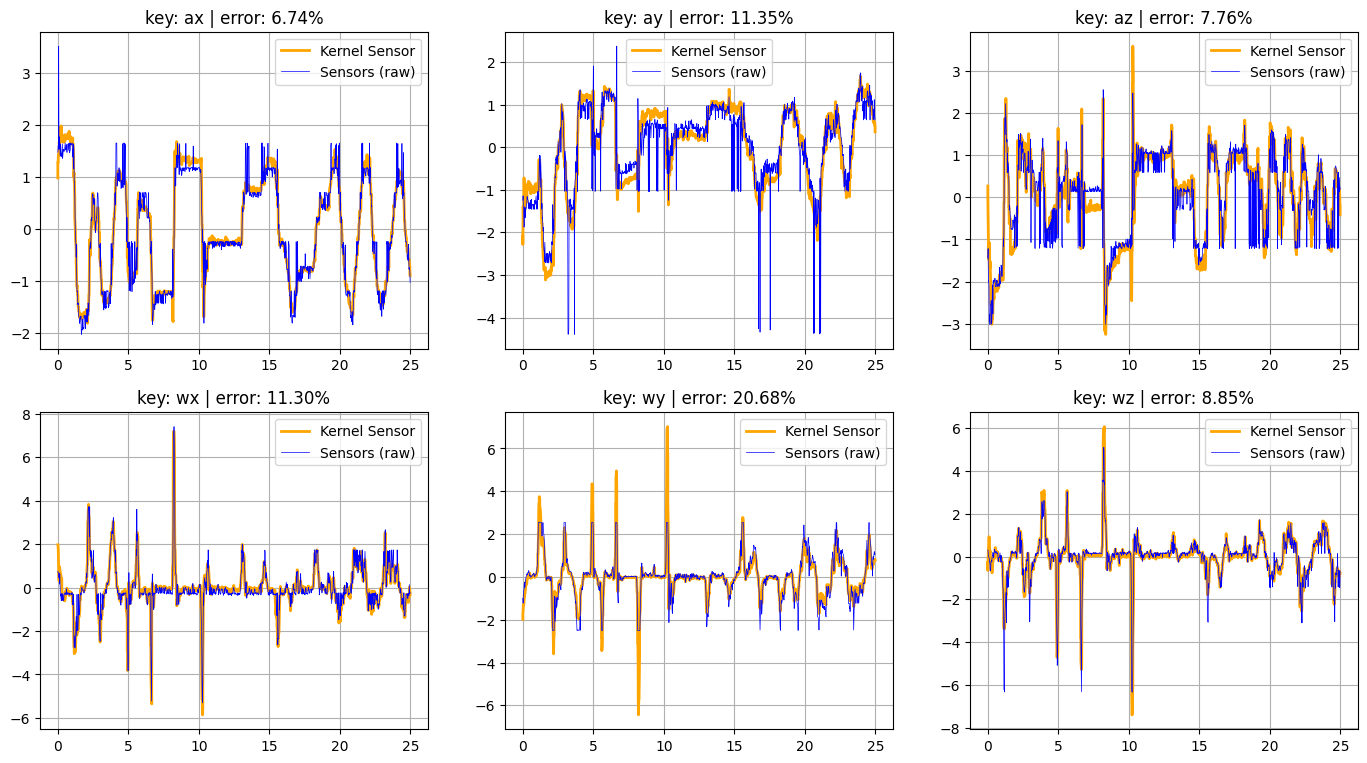
\includegraphics[width=\linewidth]{imagens/comp_raw.png}
                
                \textbf{Fonte:} Autor
                \label{fig:raw}
            \end{figure}

             A partir dessas métricas, fica evidente que o uso direto dos dados do MPU é inviável para os objetivos do projeto, e o estudo realizado anteriormente sobre filtros e algoritmos de fusão agora pode ser realizado e implementado, mas desta vez, comparado com um sensor de alta precisão, o que permite validar o modelo. Como métrica de erro para verificar a diferença entre as duas medições, foi adotada a distância de Wasserstein, que, de acordo com RÜSCHENDORF (1985), calcula o trabalho mínimo necessário para transportar uma distribuição de probabilidade para outra, sendo o resultado final convertido em uma porcentagem de erro.

        
        \subsubsection{Comparação em Modo Filtrado}
            Conforme evidenciado no relatório anterior, o filtro de Butterworth, configurado com frequência de corte de 0,5 Hz, mostrou-se mais eficaz para os sensores MPU por reduzir o ruído sem introduzir atrasos significativos que comprometesse a resposta do sistema. Diante desse resultado, os mesmos dados são representados na \autoref{fig:filter}, agora com a aplicação do referido filtro em todas as variáveis dos MPU, visando à comparação direta de seu desempenho com o sensor Kernel.

            \begin{figure}[H]
                \centering
                \caption{Comparação dos Sensores em Dados Filtrados}
                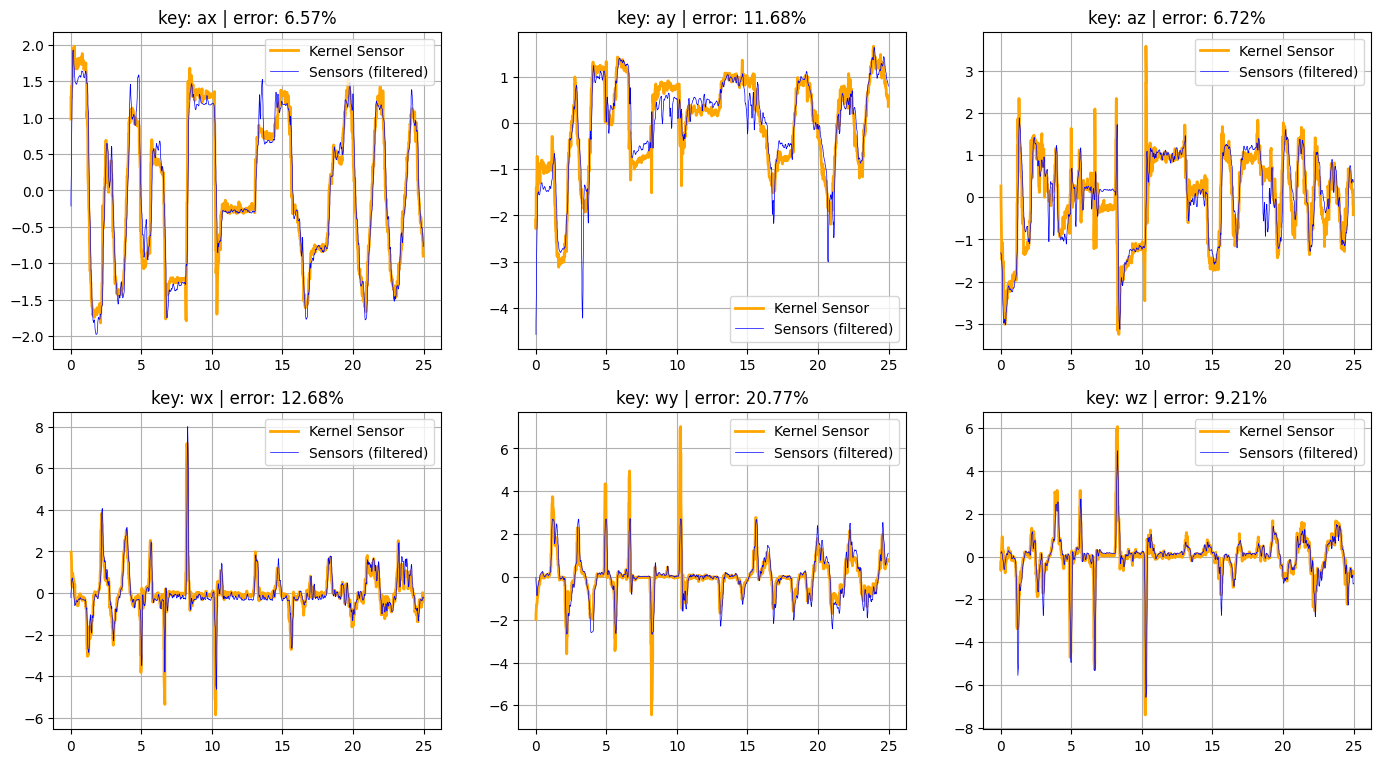
\includegraphics[width=\linewidth]{imagens/comp_filter.png}
                
                \textbf{Fonte:} Autor
                \label{fig:filter}
            \end{figure}

             A análise dos gráficos demonstra que, mesmo com os avanços na suavização e na redução de ruído dos dados filtrados, o MPU ainda apresenta limitações na detecção de variações abruptas. Diferentemente do Kernel, o sensor não identifica os picos dessas oscilações e, em alguns casos, exibe divergência ao retornar ao estado inicial, o que compromete o desempenho do sistema. Essa deficiência, no entanto, não pode ser corrigida exclusivamente por meio de filtros, uma vez que se origina das medições internas do próprio componente.


        \newpage
        \subsubsection{Comparação com Fusão de Kalman}
            Pesquisas sobre o filtro e a fusão de Kalman, frequentemente utilizados em Unidades de Medição Inercial (IMUs), agora permitem sua aplicação de maneira similar aos dados brutos obtidos de sensores. Nesse sentido, os sensores MPU6050 e MPU9250 foram integrados por meio de um algoritmo que realiza a filtragem e combinação de suas informações, gerando uma única saída passível de comparação. Dessa forma, o método foi implementado nos dispositivos, e o resultado final está ilustrado na figura.
            
            \begin{figure}[H]
                \centering
                \caption{Comparação do Kernel com MPUs (Fusão de Kalman)}
                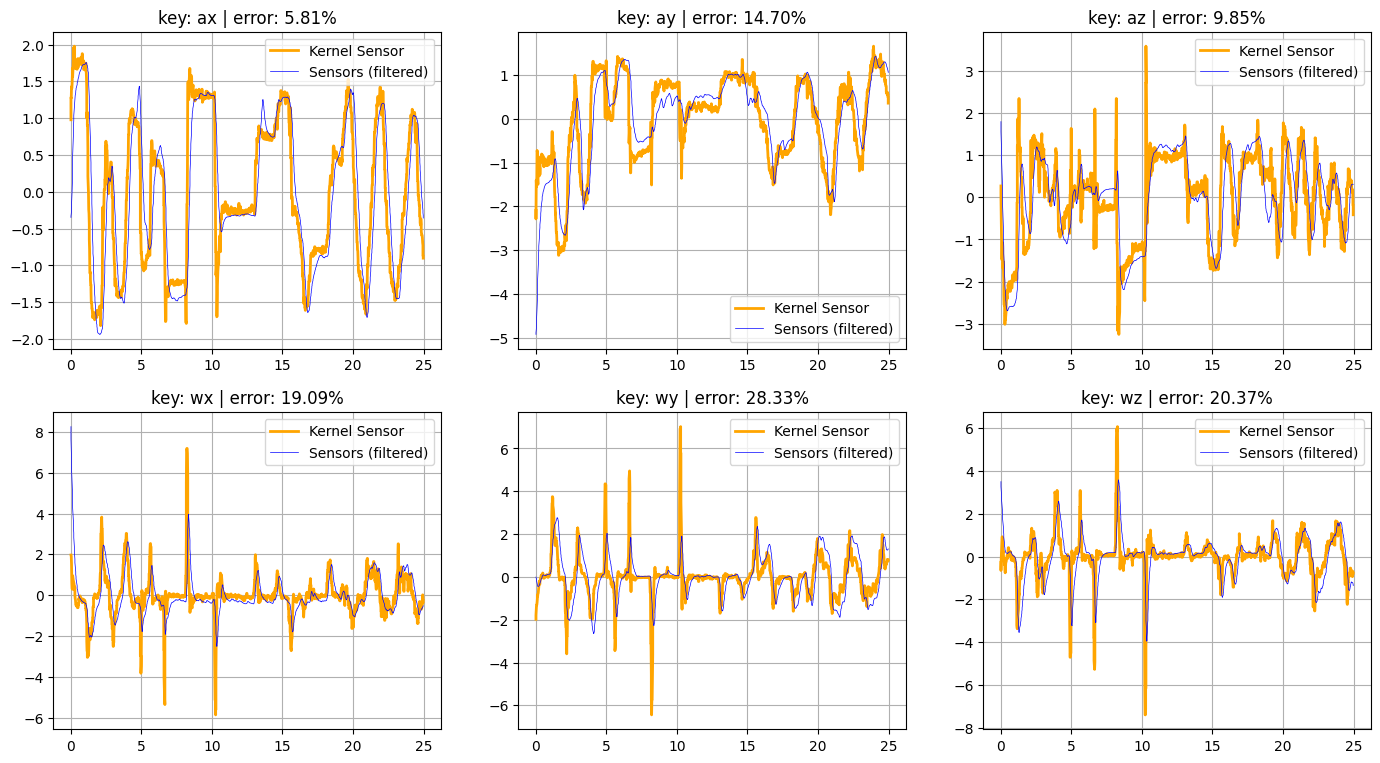
\includegraphics[width=\linewidth]{imagens/comp_fusion.png}
                
                \textbf{Fonte:} Autor
                \label{fig:placeholder}
            \end{figure}

             A análise dos dados indica que a fusão de sensores não produziu o resultado esperado na redução do erro de medição entre o sensor Kernel e os MPUs processados. Essa limitação confirma a necessidade de se adotar um sensor de maior precisão, uma vez que o problema não está relacionado a ruídos, mas sim a uma característica intrínseca do dispositivo atual. Nos testes realizados, tanto o sinal bruto quanto o filtrado demonstraram incapacidade de responder com a necessária agilidade às variações de movimento, que são adequadamente capturadas pelo sensor Kernel. Constatou-se que o aumento do nível de suavização somente ampliaria o atraso na leitura das variáveis, tornando o sensor ainda menos sensível a mudanças sutis ou bruscas.


        \newpage
        \subsection{Comparação das Variáveis de Interesse}
            Considerando os estudos anteriores explicitados na macroentrega II, sobre o cálculo das variáveis de orientação (pitch, roll e yaw) a partir aceleração e velocidade angular manipuladas por quaternions, faz-se necessária a verificação desses cálculos, inicialmente implementados nos sensores MPU, em comparação com os resultados fornecidos pelo sensor Kernel, que já disponibiliza tais variáveis por meio de seu algoritmo interno via comunicação serial. Para tanto, os dados foram coletados simultaneamente de ambos os dispositivos em tempo real, e os valores de orientação calculados a partir das formas brutas de aceleração e velocidade angular nos três eixos dos MPU-6050 foram plotados juntamente com as saídas prontas do Kernel, permitindo uma análise comparativa direta, conforme ilustrado nas figuras seguintes.
            
            \begin{figure}[H]
                \centering
                \caption{Validação dos Algoritmos de Pitch}
                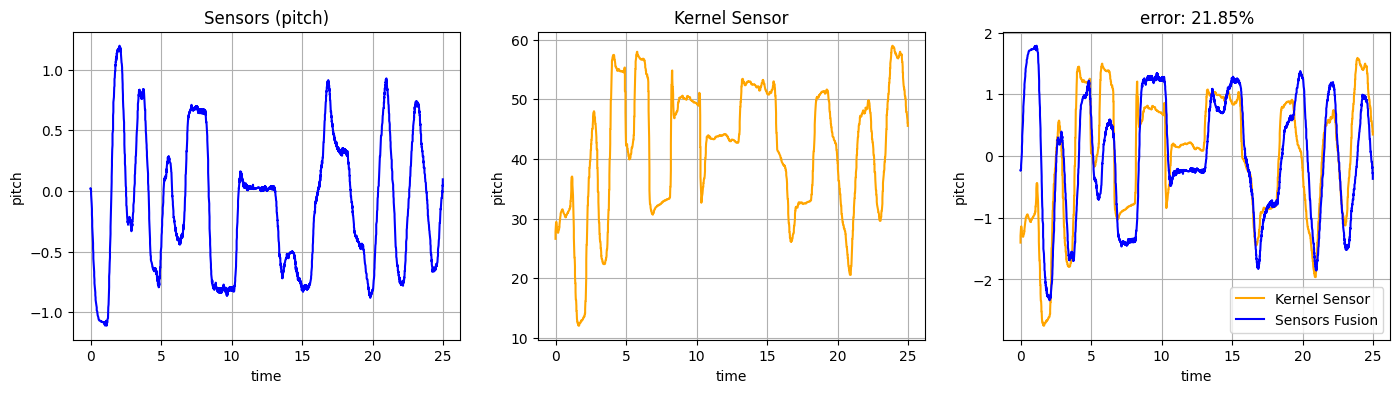
\includegraphics[width=\linewidth]{imagens/pitch_roll_yaw.png}
                
                \textbf{Fonte:} Autor
                \label{fig:placeholder}
            \end{figure}
    
            \begin{figure}[H]
                \centering
                \caption{Validação dos Algoritmos de Roll}
                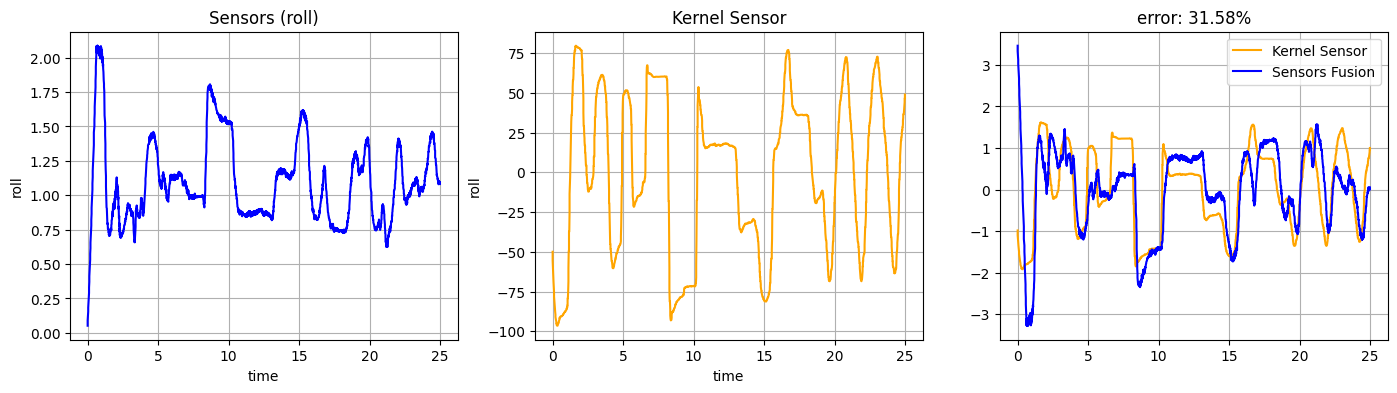
\includegraphics[width=\linewidth]{imagens/roll.png}
                
                \textbf{Fonte:} Autor
                \label{fig:placeholder}
            \end{figure}
    
            \begin{figure}[H]
                \centering
                \caption{Validação dos Algoritmos de Yaw}
                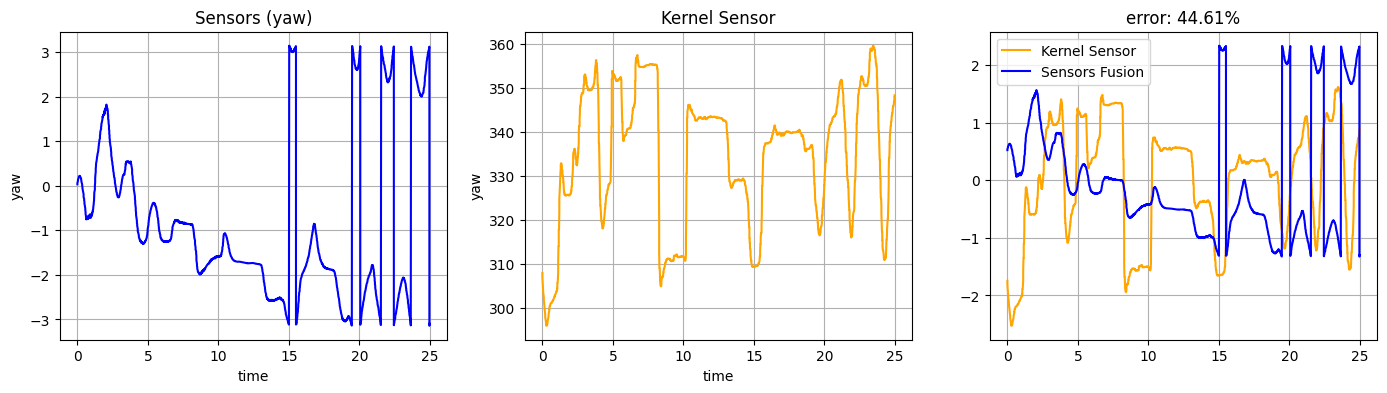
\includegraphics[width=\linewidth]{imagens/yaw.png}
                
                \textbf{Fonte:} Autor
                \label{fig:placeholder}
            \end{figure}

            Os dados indicam que, embora apresentem alta similaridade, as variáveis de orientação demonstram pequenas discrepâncias nos eixos de pitch e roll, e uma diferença significativa no yaw. Essa variação mais acentuada no yaw pode ser atribuída à imprecisão inerente aos sensores MPU, cujos erros se amplificam quando submetidos a cálculos de maior complexidade, como os envolvidos na determinação desse parâmetro específico.


    \newpage
    \subsection{Protocolo de Comunicação}
        O software de monitoramento, responsável pela aquisição dos dados provenientes do DRMM e pela sua apresentação ao usuário final, exige que as informações sejam recebidas em um formato específico, alinhado com as normativas técnicas predominantes no mercado. Consequentemente, optou-se pela implementação do protocolo NMEA 0183 (National Marine Electronics Association 0183). Esse protocolo utiliza comunicação serial assíncrona fundamentada principalmente no padrão RS-422 e é amplamente utilizado no mercado para transmissão de dados, além de ser um padrão adotado para a área em destaque, conforme mostrado por LANGLEY (1995). 
        
        O baud rate padrão da maioria dos dispositivos NMEA 0183 é 4800 bps, e possuem o
        tamanho de 8 bits sendo o último igual a zero (d7 = 0). Em um sistema NMEA 0183, cada canal de comunicação (par de fios) deve conter apenas um transmissor (talker) e pode ter até três receptores (listeners) conectados diretamente. A \autoref{fig:protocol} exemplifica a organização descrita.

        \begin{figure}[H]
            \centering
            \caption{Enter Caption}
            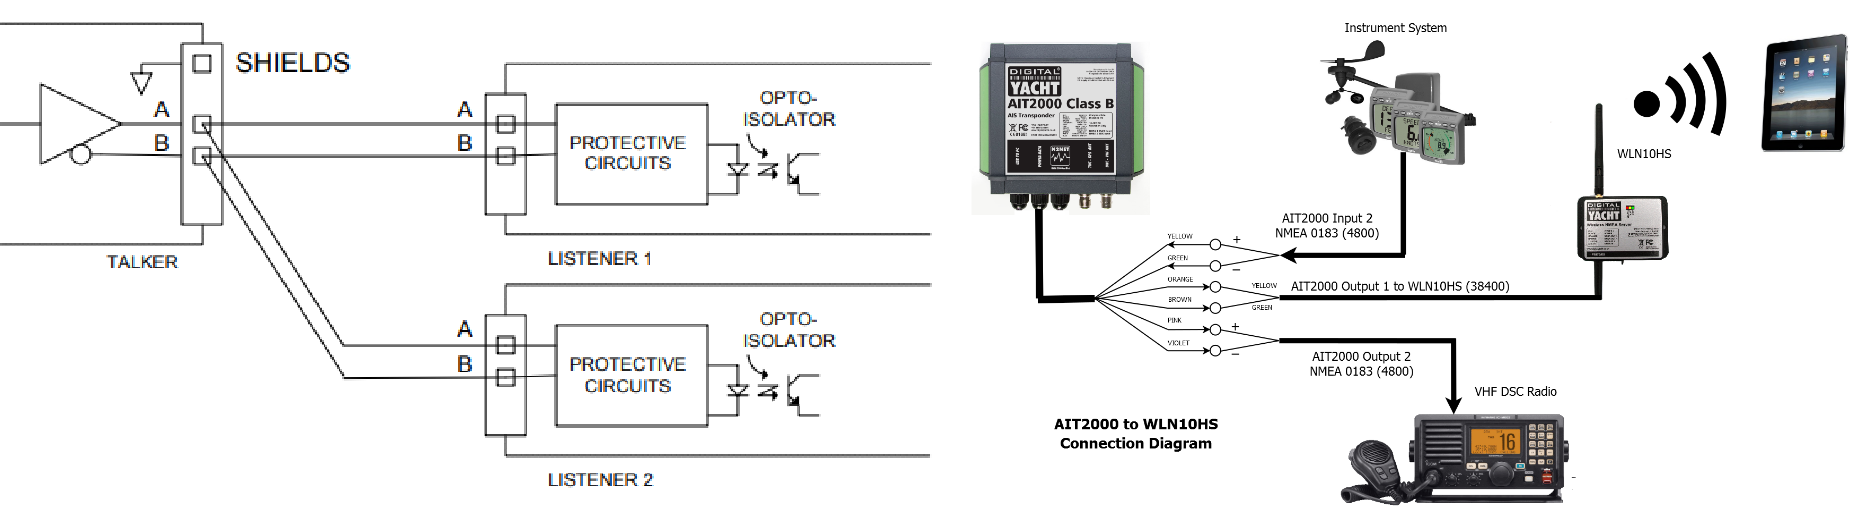
\includegraphics[width=\linewidth]{imagens/protocol.png}

            \textbf{Fonte: } CX Associates
            \label{fig:protocol}
        \end{figure}

        Mensagens em NMEA 0183 utilizam ASCII para codificar os dados, o que as tornam capazes
        de serem lidas sem a utilização de um software específico. As sentenças são divididas em campos (ou fields), com cada campo cumprindo funções específicas como identificação, dados e checagem de dados. Um campo consiste em uma string de caracteres válidos, ou não caracteres (null field), localizado entre dois caracteres delimitadores. É o primeiro campo da sentença, sempre é iniciado pelo delimitador “\$” ou “!”, eles servem para definir a sentença. O delimitador “\$” identifica a sentença convencional paramétrica, obedecendo a estrutura:

        \begin{center}
            \small
            \$<TAL\_ID><MSG\_ID>,<dados1>,<dados2>,…,<dadosN>*<checksum><CR><LF>
        \end{center}

        A \autoref{tab:protocolo} mostra a explicação de cada campo citado e como deve ser usado de forma a construir uma mensagem final com o protocolo informado.

        \begin{center}
            \centering
            {\renewcommand{\arraystretch}{1.5}
            \begin{longtable}{|c|c|c|}
                \caption{Explicação dos Campos do Protocolo} \label{tab:protocolo}\\
                \hline
                     \textbf{Parâmetro} & \textbf{Nome} & \textbf{Descrição}  \\
                \hline 
                    \fcol{.15}{\$} & 
                    \col{.25}{início} & 
                    \col{.6}{Toda sentença se inicia com o caractere \$} \\
                \hline
                    \fcol{.15}{<TAL\_ID>} & 
                    \col{.25}{ID do \textit{talker}} & 
                    \col{.6}{
                        Duas letras indicando o dispositivo ou sensor (e.g., GP se refere a GPS)
                    } \\
                \hline
                    \fcol{.15}{<MSG\_ID>} & 
                    \col{.25}{Tipo de mensagem} & 
                    \col{.6}{Três letras determinando o tipo de mensagem está sendo enviada
                        (e.g., uma mensagem RMC transmitirá dados de horário, data,
                        posição, curso e velocidade)} \\
                \hline
                    \fcol{.15}{<dados1>,..} & 
                    \col{.25}{Dados} & 
                    \col{.6}{Informações específicas da mensagem separadas por vírgula} \\
                \hline
                    \fcol{.15}{*} & 
                    \col{.25}{Fim da mensagem} & 
                    \col{.6}{Valor que identifica o fim da mensagem} \\
                \hline
                    \fcol{.15}{<checksum>} & 
                    \col{.25}{Checksum} & 
                    \col{.6}{Valor hexadecimal de 2 dígitos para a validação da integridade mensagem} \\
                \hline
                    \fcol{.15}{<CR><LF>} & 
                    \col{.25}{Fim da sentença} & 
                    \col{.6}{Caracteres de controle para quebra de linha: Carriage Return e Line Feed} \\
                \hline
                \end{longtable}
            }

            \textbf{Fonte:} Autor
        \end{center}
        
        Os parâmetros \$, TAL\_ID e MSG\_ID compõe o cabeçalho (header) da mensagem, o que
        define qual o formato da mensagem a ser enviado. Usando-se como exemplo um dispositivo de receptor de gps (talker) que tenha seu TAL\_ID como GP (Global Positioning Syst) que envie uma mensagem com o MSG\_ID sendo GGA (Global Positioning System Fixed Data), possuirá o seu header como \$GPGGA, e sua mensagem será enviada como no seguinte exemplo (SIRF TECHNOLOGY, 2007, p.9):

        \begin{center}
            \$GPGGA,002153.000,3342.6618,N,11751.3858,W,1,10,1.2,27.0,M,-34.2,M,,0000*5E
        \end{center}

        \begin{center}
        \centering
        {\renewcommand{\arraystretch}{1.5}
        \begin{longtable}{|c|c|c|c|}
            \caption{Tabela 2: Exemplo de Formato de Mensagem GGA}\label{tab:gga}\\
            \hline
            \textbf{Name} & \textbf{Example} & \textbf{Unit} & \textbf{Description} \\
            \hline
            \fcol{.2}{Message ID}              & \col{.15}{\$GPGGA}   & \col{.15}{~}     & \col{.5}{GGA protocol header} \\
            \hline
            \fcol{.2}{UTC Time}                & \col{.15}{002153.000}& \col{.15}{~}     & \col{.5}{hhmmss.sss} \\
            \hline
            \fcol{.2}{Latitude}                & \col{.15}{3342.6618} & \col{.15}{~}     & \col{.5}{ddmm.mmmm} \\
            \hline
            \fcol{.2}{N/S Indicator}           & \col{.15}{N}         & \col{.15}{~}     & \col{.5}{N=north or S=south} \\
            \hline
            \fcol{.2}{Longitude}               & \col{.15}{11751.3858}& \col{.15}{~}     & \col{.5}{dddmm.mmmmm} \\
            \hline
            \fcol{.2}{E/W Indicator}           & \col{.15}{W}         & \col{.15}{~}     & \col{.5}{E=east or W=west} \\
            \hline
            \fcol{.2}{Position Fix Indicator}  & \col{.15}{1}         & \col{.15}{~}     & \col{.5}{See Table 1-4} \\
            \hline
            \fcol{.2}{Satellites Used}         & \col{.15}{10}        & \col{.15}{~}     & \col{.5}{Range 0 to 12} \\
            \hline
            \fcol{.2}{HDOP}                    & \col{.15}{1.2}       & \col{.15}{~}     & \col{.5}{Horizontal Dilution of Precision} \\
            \hline
            \fcol{.2}{MSL Altitude}            & \col{.15}{27.0}      & \col{.15}{meters}& \col{.5}{~} \\
            \hline
            \fcol{.2}{Units}                   & \col{.15}{M}         & \col{.15}{meters}& \col{.5}{~} \\
            \hline
            \fcol{.2}{Geoid Separation}        & \col{.15}{-34.2}     & \col{.15}{meters}& \col{.5}{Geoid-to-ellipsoid separation. Ellipsoid altitude = MSL Altitude + Geoid Separation.} \\
            \hline
            \fcol{.2}{Units}                   & \col{.15}{M}         & \col{.15}{meters}& \col{.5}{~} \\
            \hline
            \fcol{.2}{Age of Diff. Corr.}      & \col{.15}{~}         & \col{.15}{sec}   & \col{.5}{Null fields when DGPS is not used} \\
            \hline
            \fcol{.2}{Diff. Ref. Station ID}   & \col{.15}{0000}      & \col{.15}{~}     & \col{.5}{~} \\
            \hline
            \fcol{.2}{Checksum}                & \col{.15}{*5E}       & \col{.15}{~}     & \col{.5}{~} \\
            \hline
            \fcol{.2}{\textless CR\textgreater\textless LF\textgreater} &
            \col{.15}{~} & \col{.15}{~} & \col{.5}{End of message termination} \\
            \hline
        \end{longtable}
        }
    
        \textbf{Fonte:} SiRF Technology, Inc, 2007
    \end{center}

    
    \begin{center}
        \centering
        {\renewcommand{\arraystretch}{1.5}
        \begin{longtable}{|c|c|}
            \caption{Tabela 2.1: Position Fix Indicator (referido como Tabela 1-4)}\label{tab:pos-fix}\\
            \hline
            \textbf{Valor} & \textbf{Descrição} \\
            \hline
            \fcol{.3}{0} & \col{.7}{Fix not valid} \\
            \hline
            \fcol{.3}{1} & \col{.7}{GPS fix} \\
            \hline
            \fcol{.3}{2} & \col{.7}{Differential GPS fix (DGNSS), SBAS, OmniSTAR VBS, Beacon, RTX in GVBS mode} \\
            \hline
            \fcol{.3}{3} & \col{.7}{Not applicable} \\
            \hline
            \fcol{.3}{4} & \col{.7}{RTK Fixed, xFill} \\
            \hline
            \fcol{.3}{5} & \col{.7}{RTK Float, OmniSTAR XP/HP, Location RTK, RTX} \\
            \hline
            \fcol{.3}{6} & \col{.7}{INS Dead reckoning} \\
            \hline
        \end{longtable}
        }
    
        \textbf{Fonte:} SiRF Technology, Inc, 2007
    \end{center}

    \begin{center}
        \centering
        {\renewcommand{\arraystretch}{1.5}
        \begin{longtable}{|c|c|}
            \caption{Tabela 3: Sentenças enviadas por um dispositivo OxTS}\label{tab:oxts-sentencas}\\
            \hline
            \textbf{Type} & \textbf{Name} \\
            \hline
            \fcol{.3}{GGA}   & \col{.7}{Geographical Fix Information} \\
            \hline
            \fcol{.3}{HDT}   & \col{.7}{Heading True} \\
            \hline
            \fcol{.3}{ZDA}   & \col{.7}{Date and Time} \\
            \hline
            \fcol{.3}{VTG}   & \col{.7}{Velocity and Track over Ground} \\
            \hline
            \fcol{.3}{GST}   & \col{.7}{GPS Pseudorange Noise Statistics} \\
            \hline
            \fcol{.3}{RMC}   & \col{.7}{Recommended Minimum data for GPS} \\
            \hline
            \fcol{.3}{PASHR} & \col{.7}{Heading, Pitch, Roll} \\
            \hline
            \fcol{.3}{GSV}   & \col{.7}{GPS Satellites in view} \\
            \hline
            \fcol{.3}{GSA}   & \col{.7}{GPS DOP and active satellites} \\
            \hline
            \fcol{.3}{PTCF}  & \col{.7}{Orientation and angular rate} \\
            \hline
        \end{longtable}
        }
    
        \textbf{Fonte:} OXFORD TECHNICAL SOLUTIONS (OxTS) (2010)
    \end{center}

    O valor da soma de verificação, checksum, é obtido aplicando a operação ou exclusivo (XOR) a todos os caracteres desde o primeiro após o símbolo "\$" até o que antecede o separador "*". Para exemplificar o procedimento, é apresentado um código simples em linguagem C++ que calcula a estrutura do protocolo e utiliza o operador "\^" para realizar a operação ou exclusivo.

\begin{minted}{arduino}
const char* getINFO(void) {
    static char sentence[79 + 1]; // parte entre $ e * (sem checksum)
    static char nmea[82 + 1];     // sentença completa com $...*XX\r\n

    const char *msg_id        = "GPGGA";
    const char *utc_time      = "002153.000";
    const double latitude     = 3342.6618;   // ddmm.mmmm
    const char ns_indicator   = 'N';
    const double longitude    = 11751.3858;  // dddmm.mmmm
    const char ew_indicator   = 'W';
    const int fix_indicator   = 1;
    const int satellites_used = 10;          // 0–12
    const float hdop          = 1.2f;
    const float msl_altitude  = 27.0f;       // metros
    const char alt_units      = 'M';
    const float geoid_sep     = -34.2f;      // metros
    const char geoid_units    = 'M';
    const char *age_diff_corr = "";          // vazio se DGPS não usado
    const char *station_id    = "0000";

    snprintf(
        sentence, sizeof(sentence),
        "%s,%s,%.4f,%c,%.4f,%c,%d,%d,%.1f,%.1f,%c,%.1f,%c,%s,%s",
        msg_id, utc_time, latitude, ns_indicator, longitude, ew_indicator,
        fix_indicator, satellites_used, hdop, msl_altitude, alt_units,
        geoid_sep, geoid_units, age_diff_corr, station_id
    );

    unsigned char checksum = 0;
    for (int i=0; i<len; i++) 
        checksum ^= (unsigned char) sentence[i];
    
    snprintf(nmea, sizeof(nmea), "$%s*%02X\r\n", sentence, csum);
    return nmea;
}
\end{minted}

    \newpage
    \subsection{Software de Monitoramento}
        O software para monitoramento das variáveis de interesse foi desenvolvido utilizando React, uma biblioteca JavaScript destinada à criação de interfaces web, combinado com Tauri, um framework que possibilita a construção de aplicativos desktop nativos para sistemas como Windows, macOS e Linux, empregando tecnologias web como HTML, CSS e JavaScript em conjunto com Rust para operações de backend. Essa integração, feita apenas para testes, permite a extração em tempo real de dados de comunicação serial UART (Universal Asynchronous Receiver-Transmitter) e sua incorporação à interface do usuário, resultando em uma aplicação desktop eficaz para monitoramento. As figuras seguintes apresentam a interface preliminar do aplicativo, que já se encontra em utilização prática.

        \begin{figure}[H]
            \centering
            \caption{Software de Monitoramento (Apenas para Testes)}
            
            \subfloat[Monitoramento Gráfico]{
                \frame{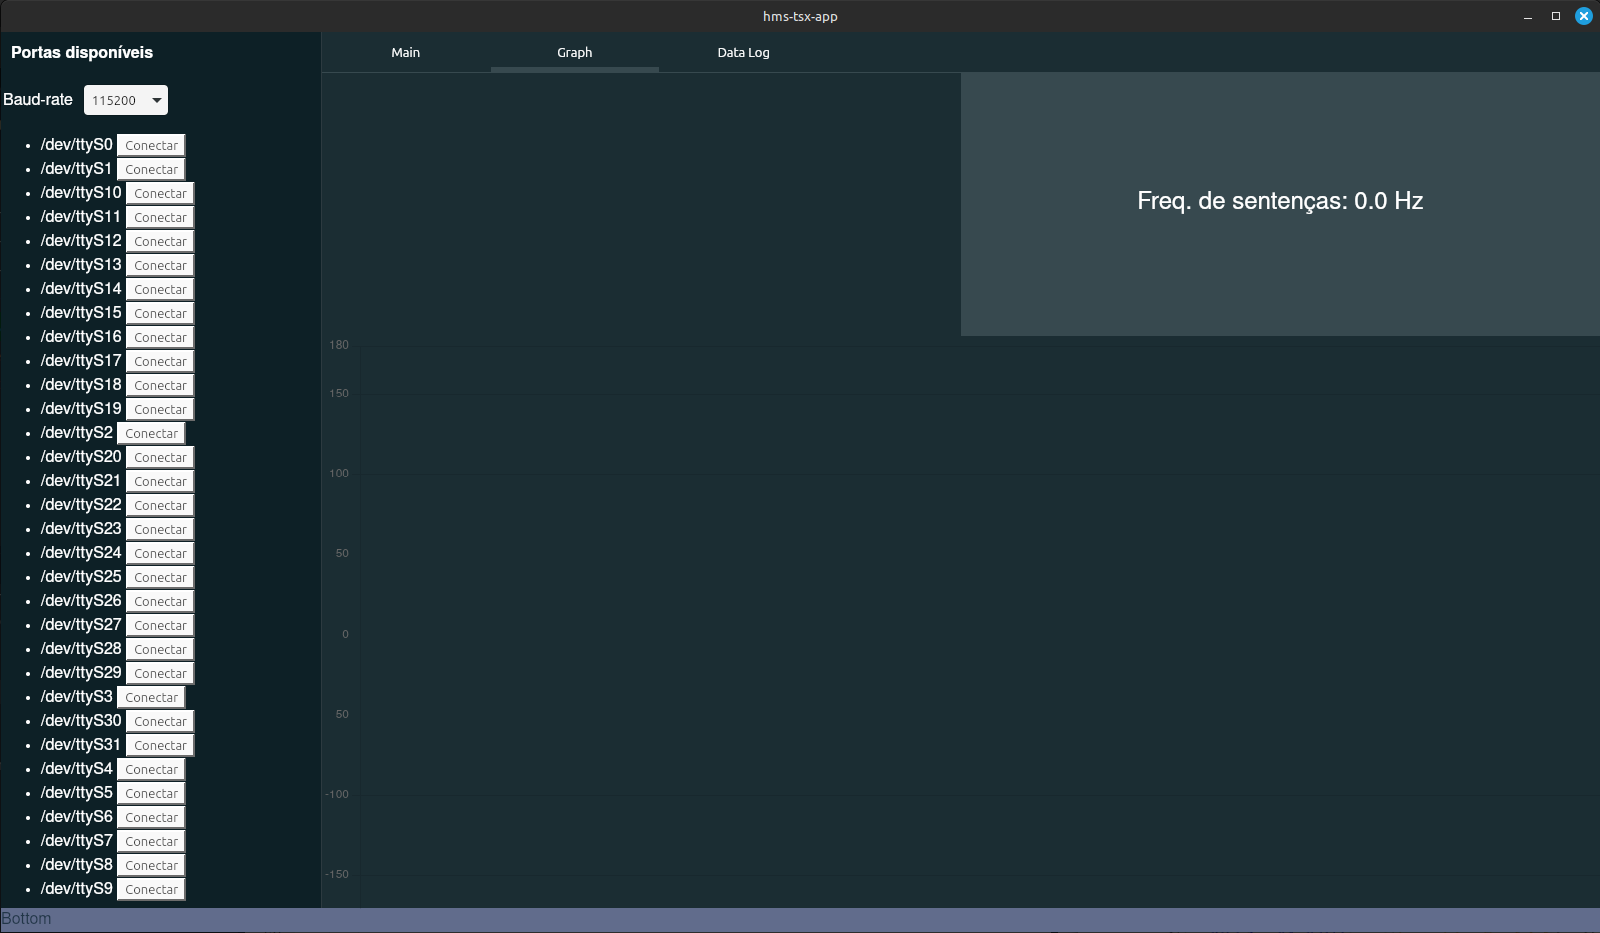
\includegraphics[width=0.5\linewidth]{imagens/hms1.png}}
                \label{fig:hmsa}
            }
            \subfloat[Monitoramento 3D]{
                \frame{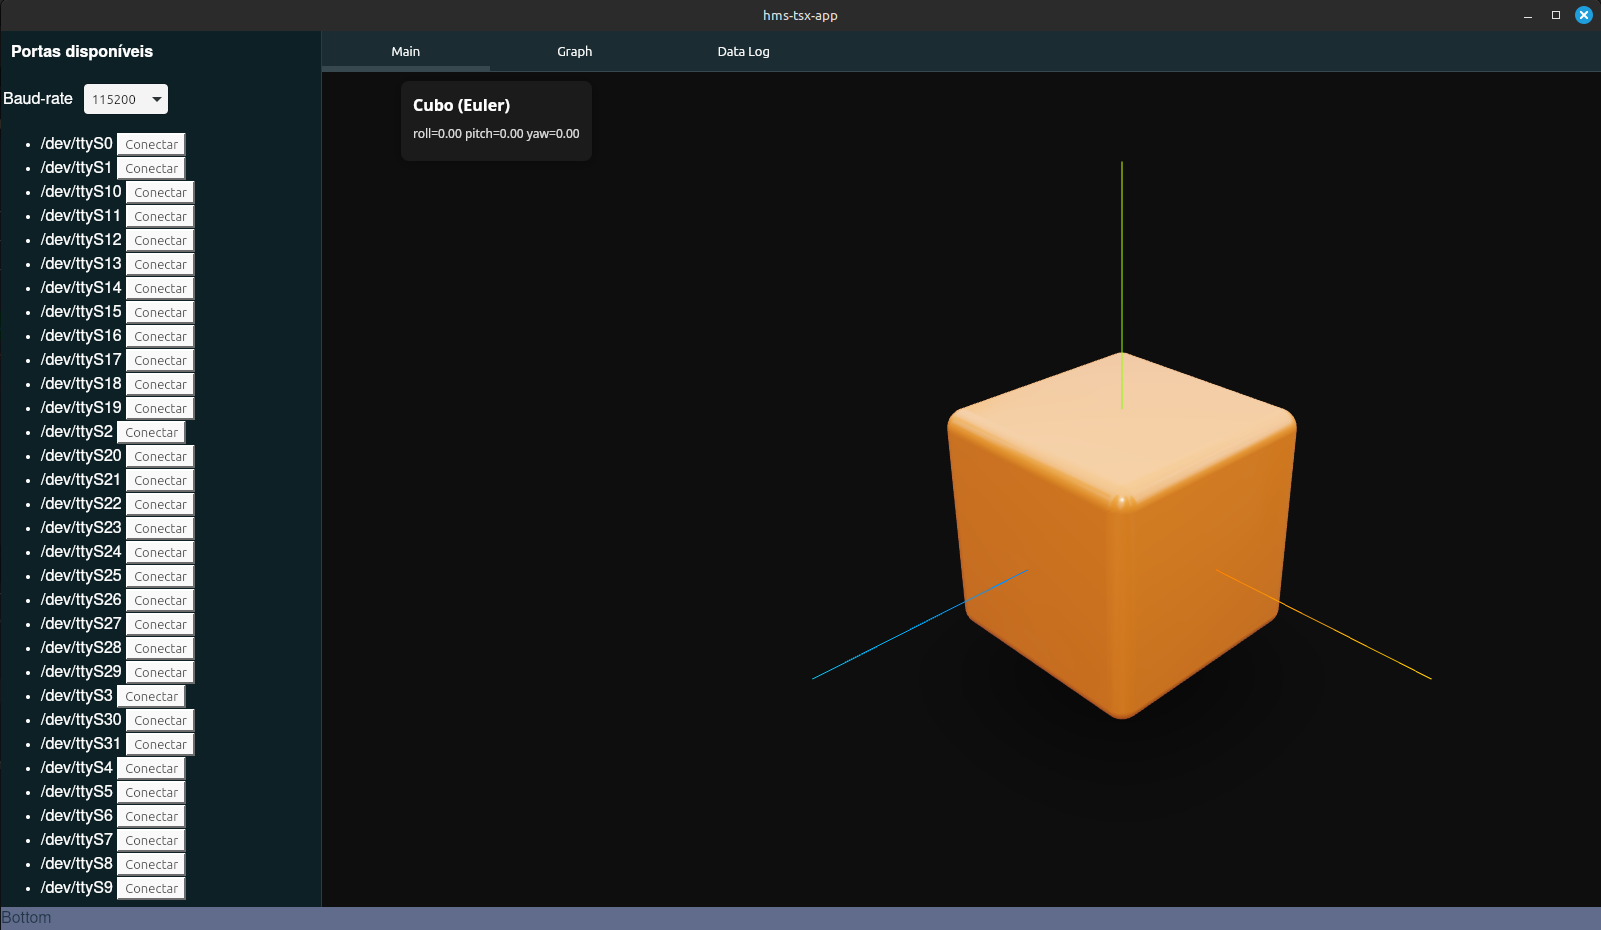
\includegraphics[width=0.5\linewidth]{imagens/hms2.png}}
                \label{fig:hmsb}
            }
            
            \subfloat[Funcionamento]{
                \frame{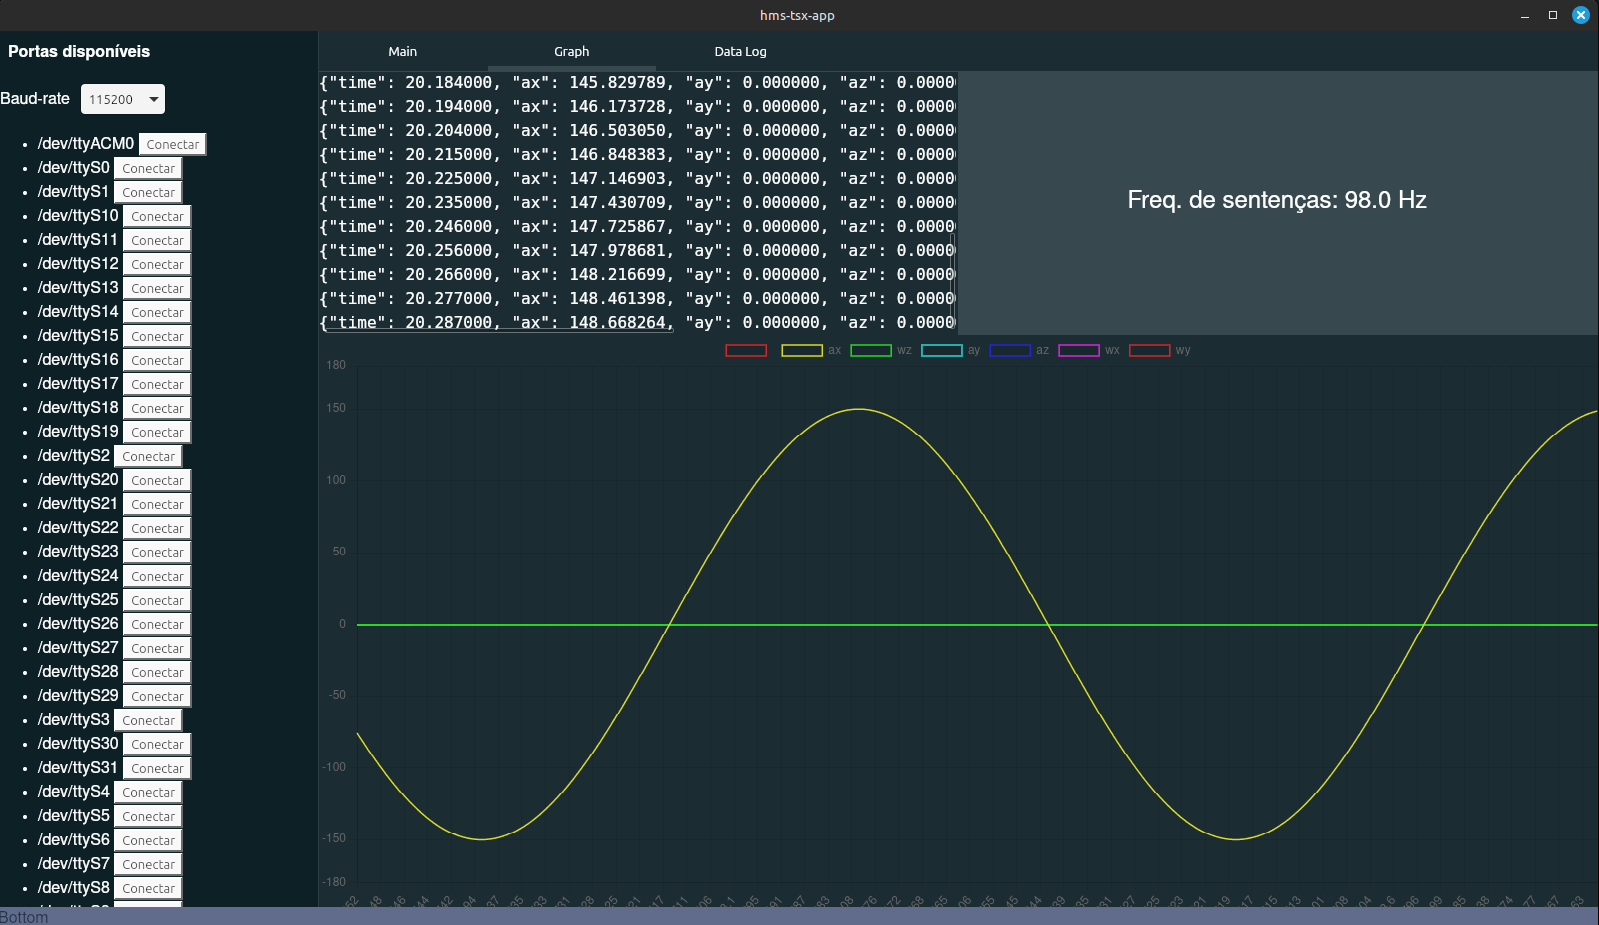
\includegraphics[width=.75\linewidth]{imagens/Screenshot from 2025-10-09 15-26-10.png}}
            }

            \textbf{Fonte:} Autor
            \label{fig:hms}
        \end{figure}

        A Figura\autoref{fig:hmsa} apresenta a interface de monitoramento linear das variáveis, que utiliza um gráfico de sequência temporal com o tempo, em segundos, no eixo das abscissas, servindo como base comum para todas as medições. No eixo das ordenadas, são plotadas as grandezas de interesse, possibilitando a visualização simultânea de seu comportamento ao longo do tempo e a comparação entre duas ou mais delas por meio de linhas individuais. O programa requer que o usuário selecione a porta de comunicação serial (COM) na qual o dispositivo está conectado; após o recebimento dos primeiros dados, as variáveis são automaticamente plotadas e inseridas na interface gráfica.

        A Figura\autoref{fig:hmsb} apresenta um modo de visualização interativa, denominado visualização de posição 3D, simbolizada por um cubo com eixos cartesianos. Essa representação permite acompanhar em tempo real a resposta do sensor aos movimentos de inclinação do sistema, que são replicados pela rotação do objeto gráfico. Embora não forneça dados precisos sobre as variáveis medidas, esse recurso é amplamente empregado no teste de Inercial Measurement Units (IMUs), pois possibilita uma verificação rápida do funcionamento do dispositivo. Dessa forma, o usuário pode configurá-lo de modo simples para uma avaliação qualitativa inicial.
        
        A validação do módulo de monitoramento ocorreu por meio da transmissão de dados no formato JSON (JavaScript Object Notation), no qual as variáveis de interesse correspondiam às chaves de cada registro enviado do Raspberry Pi ao computador via comunicação UART. Os dados foram apresentados visualmente como gráficos de linha, comprovando o correto funcionamento do sistema.
        
        \begin{figure}[H]
            \centering
            \caption{Teste do Software de Monitoramento em Bancada}
            \frame{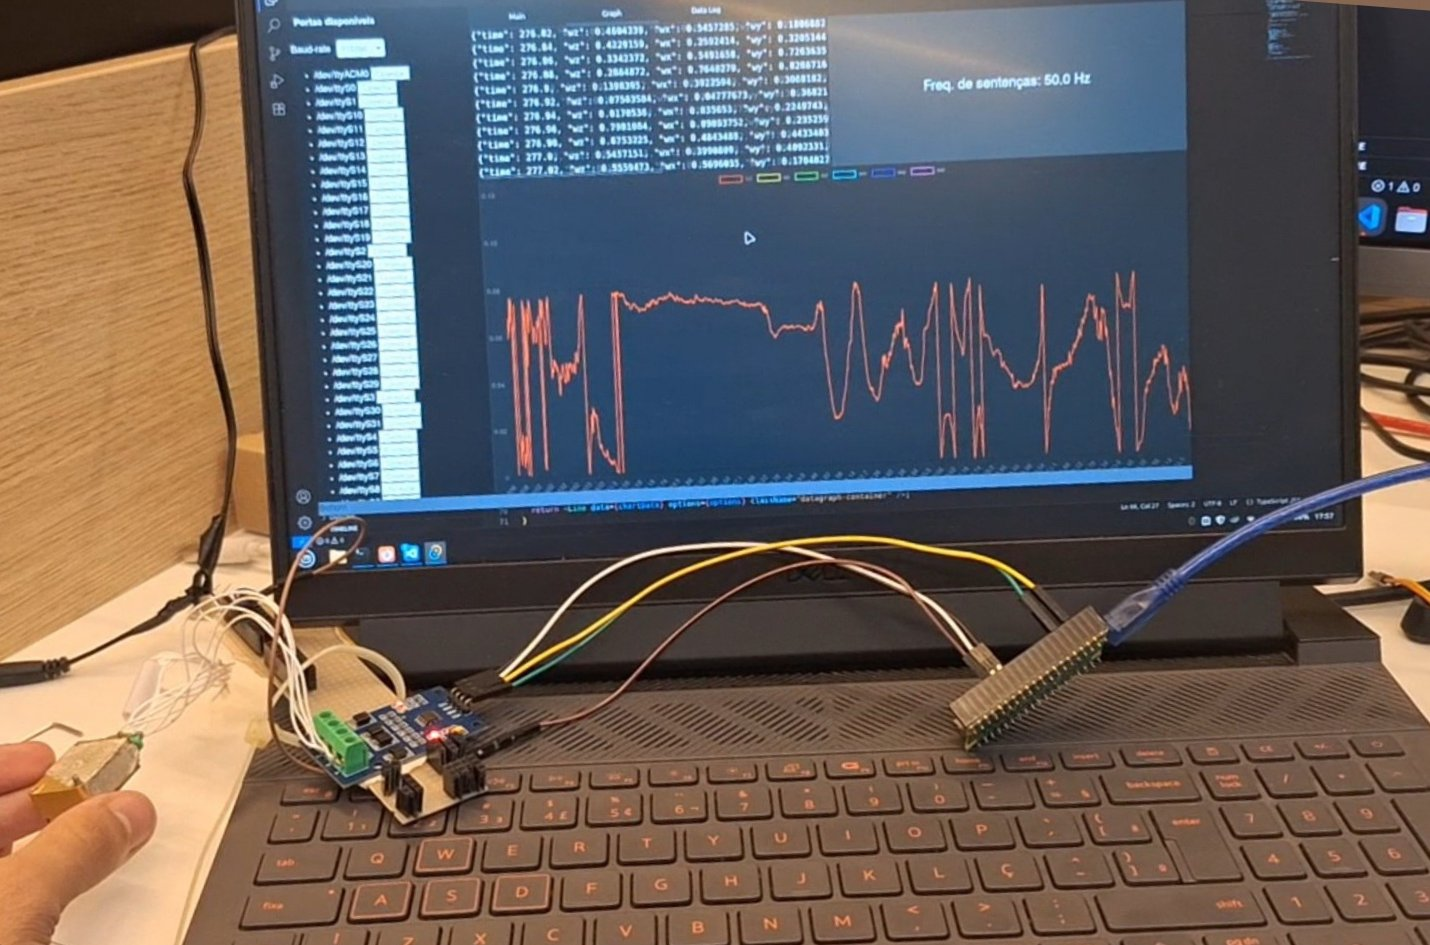
\includegraphics[width=\linewidth]{imagens/imu.jpg}}

            \textbf{Fonte:} Autor
            \label{fig:placeholder}
        \end{figure}

        O próximo passo consiste em aplicar a mesma lógica, porém incorporando o protocolo de comunicação específico estudado no projeto. Nessa perspectiva, ajustes adicionais na interface do usuário poderão ser realizados para refinamento e customização do produto final que será entregue ao parceiro.

    \subsubsection{Software de Produção (HMS)}
        O software explicado anteriormente atuou exclusivamente no monitoramento básico de variáveis para fins de teste, permitindo a validação de funções e algoritmos por meio de visualização gráfica. Para isso, a plataforma de testes foi adaptada para uma interface gráfica mais intuitiva, e alinhada à experiência comum em aplicativos desktop do setor que utilizam IMUs (Unidades de Medição Inercial, na sigla em inglês). A figura abaixo apresenta o ambiente de software produzido, denominado HMS, incluindo telas e recursos de interface desenhados para operação em ambientes offshore.

        \begin{figure}[H]
            \centering
            \caption{Telas do HMS}
            \frame{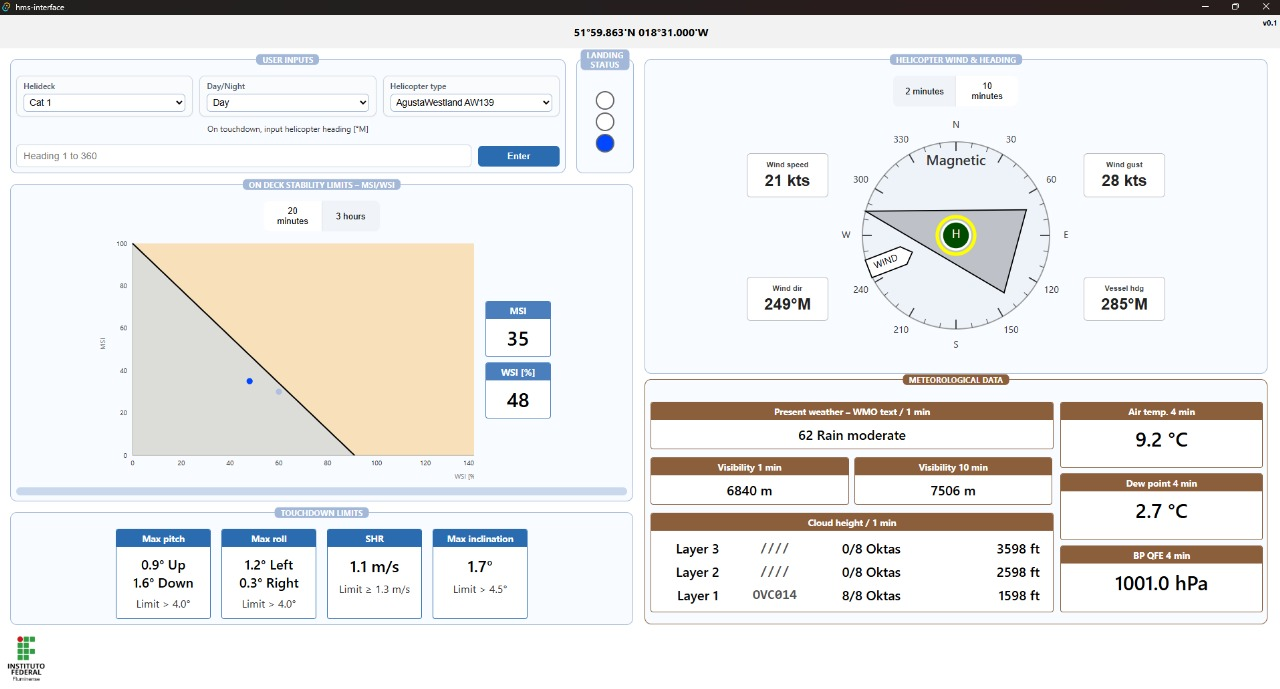
\includegraphics[width=\linewidth]{imagens/hms.jpeg}}

            \textbf{Fonte:} Autor
            \label{fig:placeholder}
        \end{figure}

        Além da visualização gráfica, similar ao software de monitoramento, a interface gráfica conta também com indicação numérica das variáveis, na forma simples e em tabela, como também uma bússola de orientação, amplamente usada para indicação de posição em softwares similares no mercado. O aplicativo também conta com parametrização em tempo real, filtros de pesquisa e indicadores de velocidade, temperatura e inclinação. 



\newpage
\section{Conclusão} 
    Portanto, todos os entregáveis referentes à macroentrega III foram concluídos com êxito, abrangendo desde a parte física até a programação. O projeto encontra-se em fase adiantada, com a construção e avaliação dos primeiros protótipos, o que permitiu testar e comparar diferentes sensores de movimento, validar seu desempenho e escolher o mais adequado para a aplicação. O sensor Kernel mostrou-se o mais preciso para capturar variáveis de movimento, apresentando resistência e resultados confiáveis tanto em movimentos abruptos quanto suaves, condições típicas em ambientes offshore. 
    
    Enquanto isso, os sensores da família MPU, embora não tenham sido os selecionados para o produto final, serviram como base para desenvolver e ajustar os algoritmos de filtragem e fusão de dados, utilizando o Kernel como parâmetro de comparação. Dessa forma, foi possível definir as melhores técnicas de processamento, que agora serão implementadas no sensor Kernel escolhido.

\newpage
\newpage

% ATIVA O CABEÇALHO DAS REFERÊNCIAS
\pagestyle{modeloReferencias}

% ADICIONA UM TIPO "SECTION" CUSTOMIZADO NO SUMÁRIO
\addcontentsline{toc}{section}{Referências}

% CRIA UMA SECTION SEM NUMERAÇÃO
\section*{Referências}
\vspace{-.5cm}
%\hyperlink{MARINHA}{(MARINHA, 2017)}

\vspace{.5cm}\noindent
JIAN, Huang. Design of angle detection system based on MPU6050. In: 7th International Conference on Education, Management, Information and Computer Science (ICEMC 2017). Atlantis Press, 2016. p. 6-8.

\vspace{.5cm}\noindent
LANGLEY, Richard. Nmea 0183: A gps receiver. GPS world, v. 6, n. 7, p. 54-57, 1995.

\vspace{.5cm}\noindent
KOMARY, Mahyad et al. Developing and validation of an inclinometer sensor based on fusion of a magnetometer, an accelerometer and a gyroscope sensor for SHM applications. In: Bridge Safety, Maintenance, Management, Life-Cycle, Resilience and Sustainability. CRC Press, 2022. p. 1607-1611.

\vspace{.5cm}\noindent
RÜSCHENDORF, Ludger. The Wasserstein distance and approximation theorems. Probability Theory and Related Fields, v. 70, n. 1, p. 117-129, 1985.

\vspace{.5cm}\noindent
SIRF TECHNOLOGY, Inc. NMEA Reference Manual – Rev. 2.1. Dez. 2007. Disponível em:
<\url{https://cdn.sparkfun.com/assets/a/3/2/f/a/NMEA_Reference_Manual-Rev2.1-Dec07.pdf}> Acesso
em: 17 maio 2025.

\phantom{a}
\newpage
    \thispagestyle{empty}
    \centering
    \phantom{a}
    \vfill

    \addcontentsline{toc}{section}{Anexos}
    \Large
    \textbf{Anexos}
    
    \vfill
    \phantom{a}
\newpage

\begin{figure}[H]
    \centering
    \caption{Desenho Técnico Compartimento - Tampa Superior}
    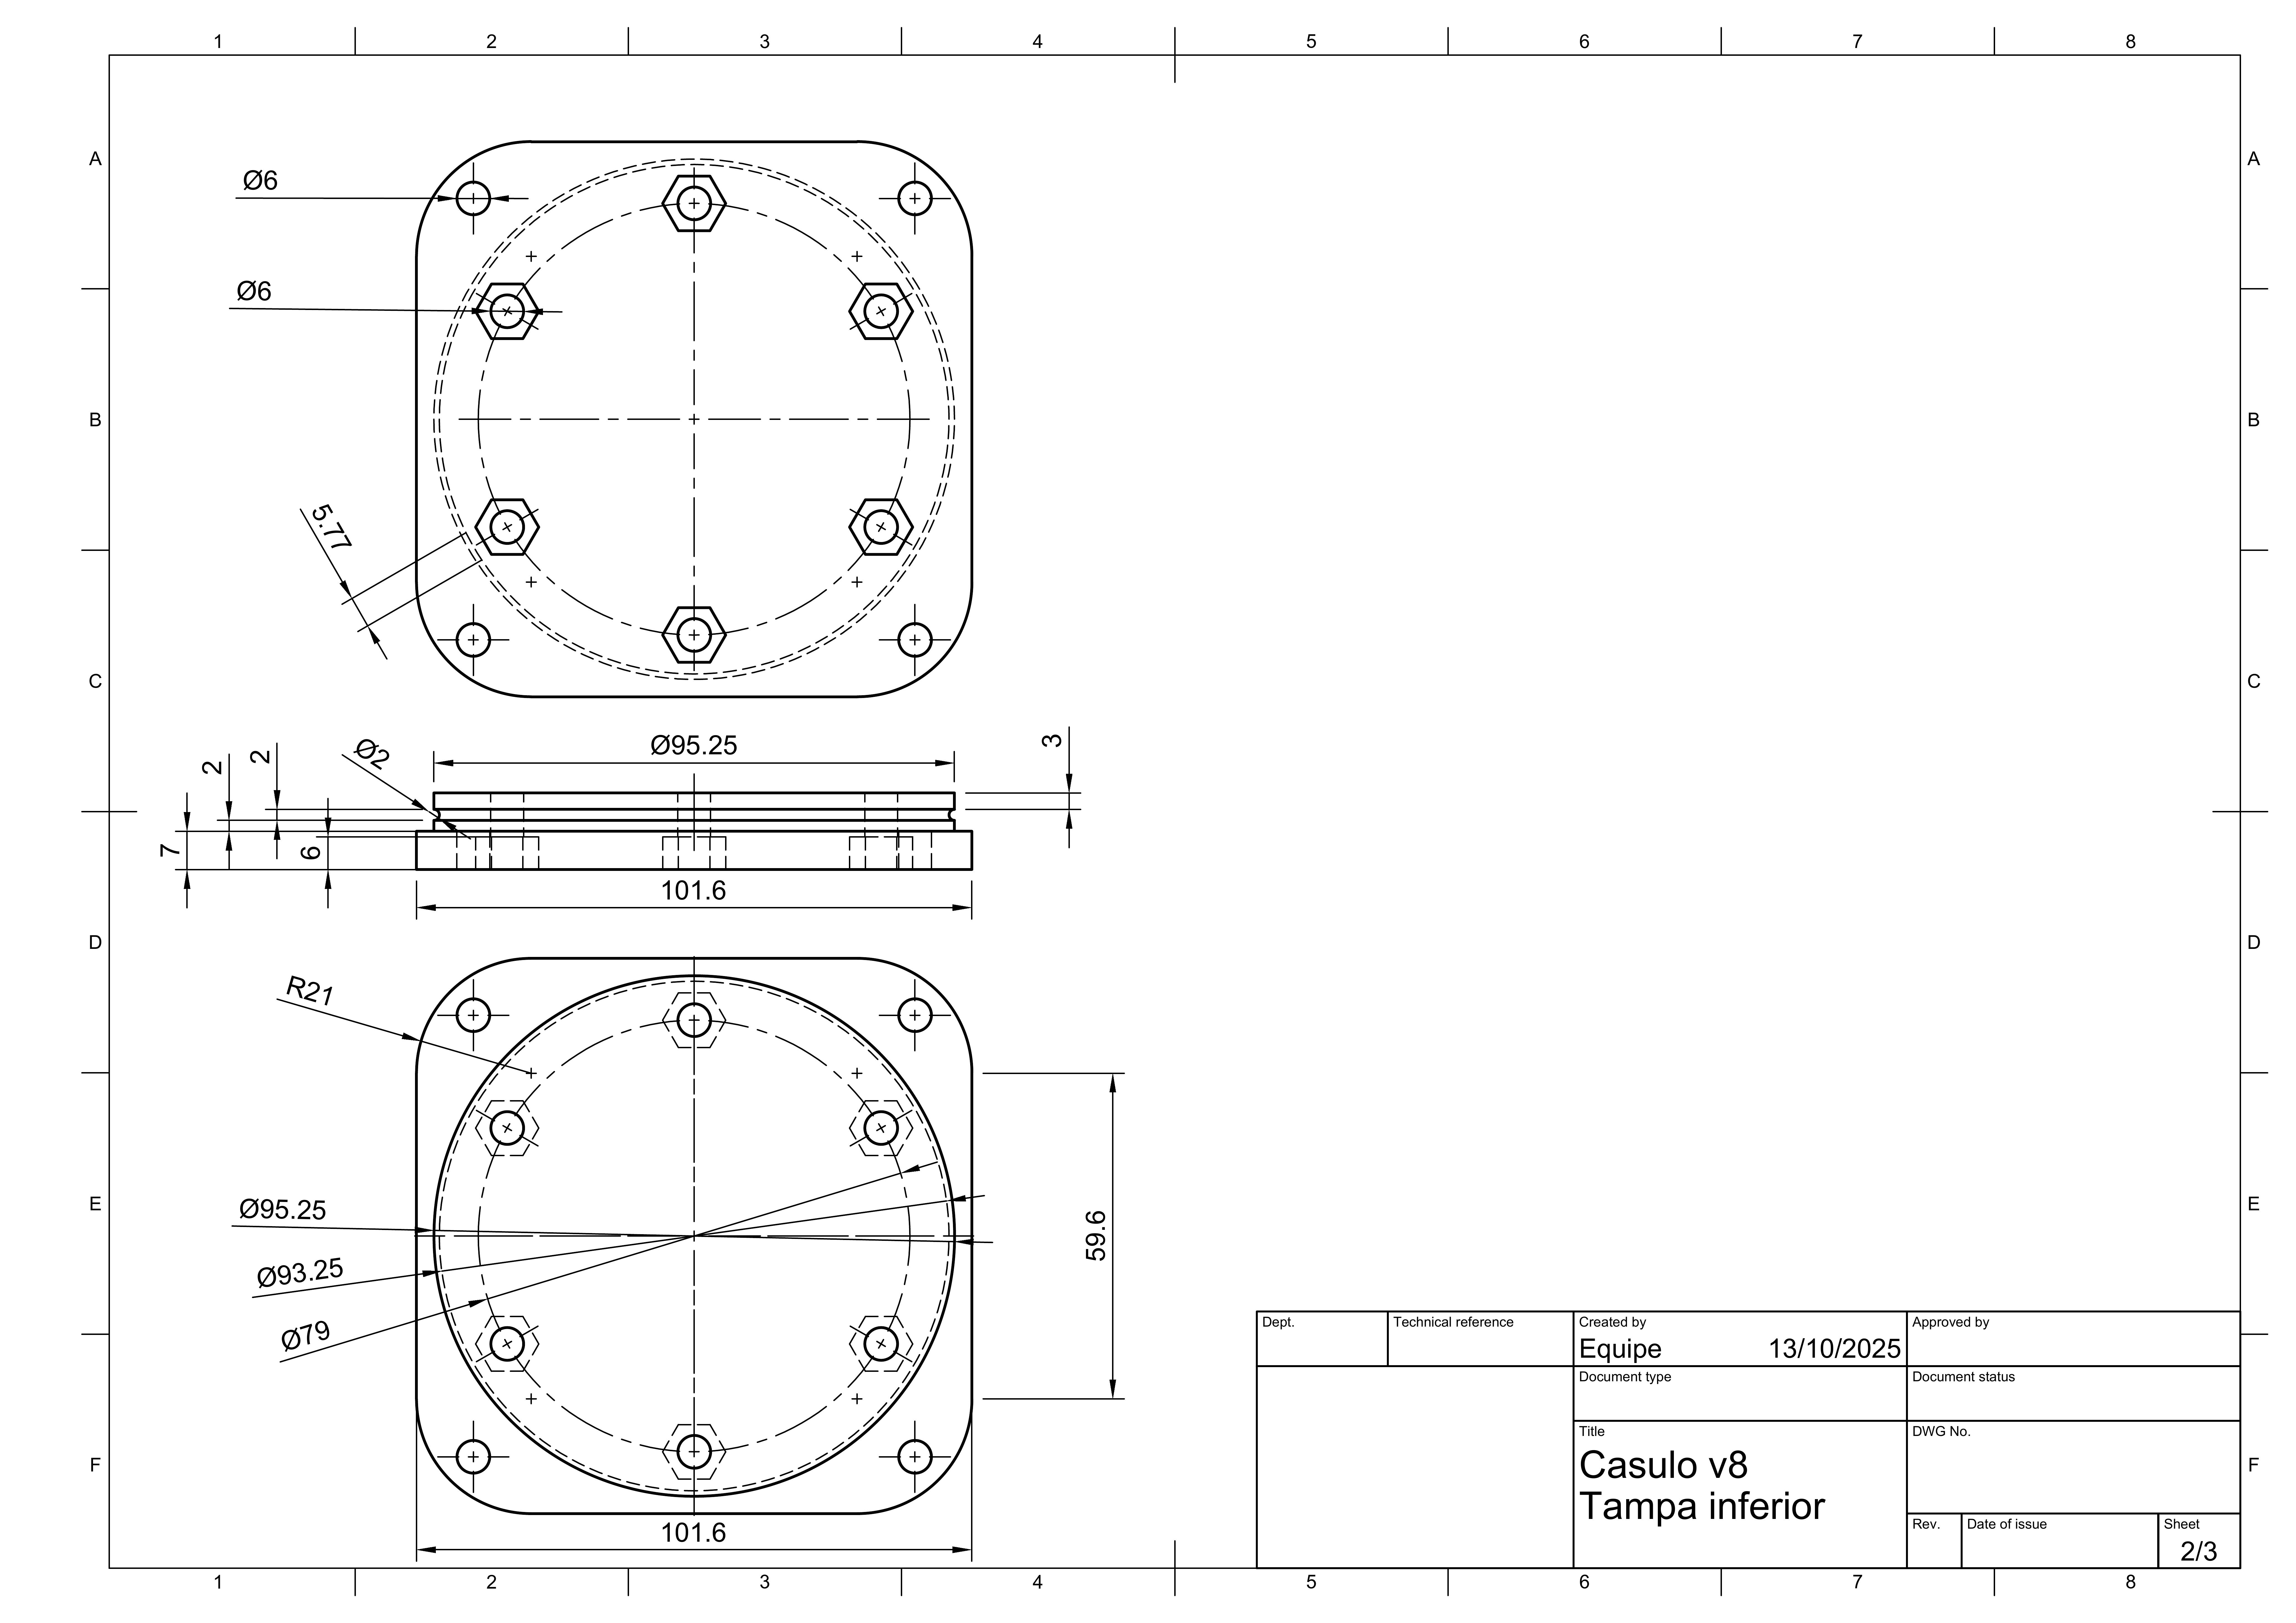
\includegraphics[width=.95\linewidth]{imagens/desenho_anexo_4.png}
    
    \label{fig:enter-label}
    \textbf{Fonte: } Autor
\end{figure}

\begin{figure}[H]
    \centering
    \caption{Desenho Técnico Compartimento - Tampa Inferior}
    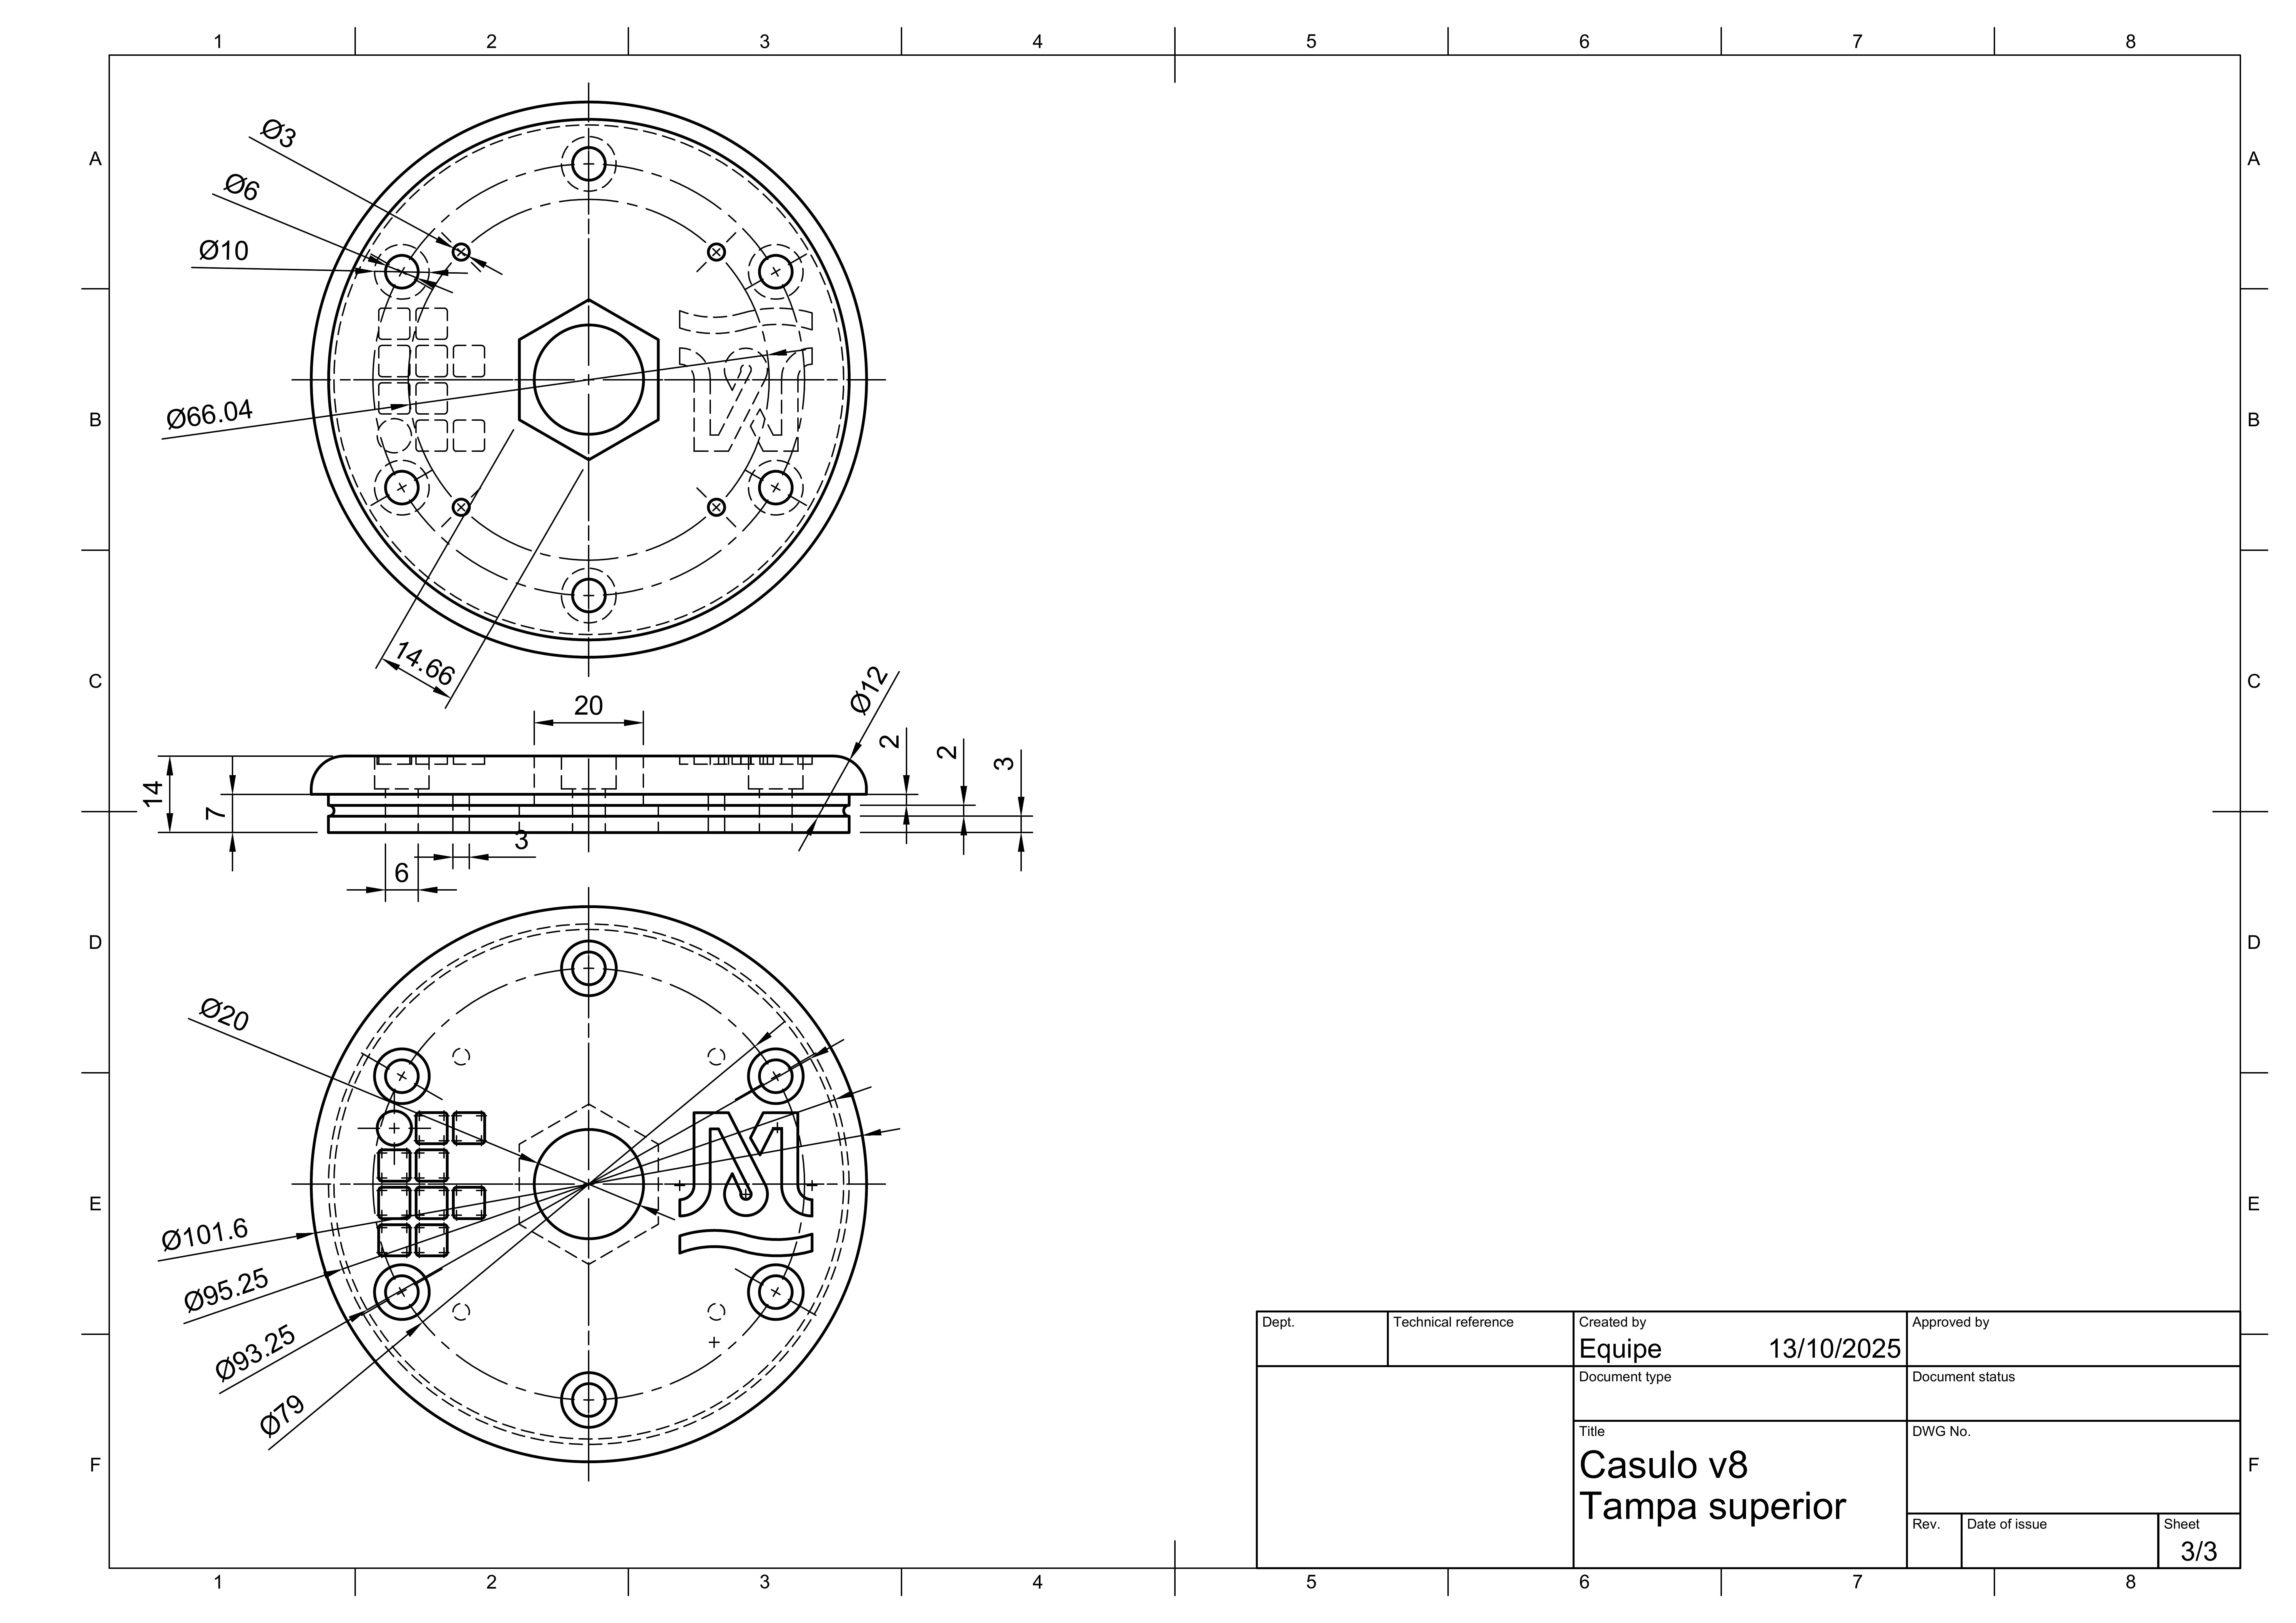
\includegraphics[width=.95\linewidth]{imagens/desenho_anexo_5.png}
    
    \label{fig:enter-label}
    \textbf{Fonte: } Autor
\end{figure}

\begin{figure}[H]
    \centering
    \caption{Desenho Técnico Compartimento - Tampa Cilindro}
    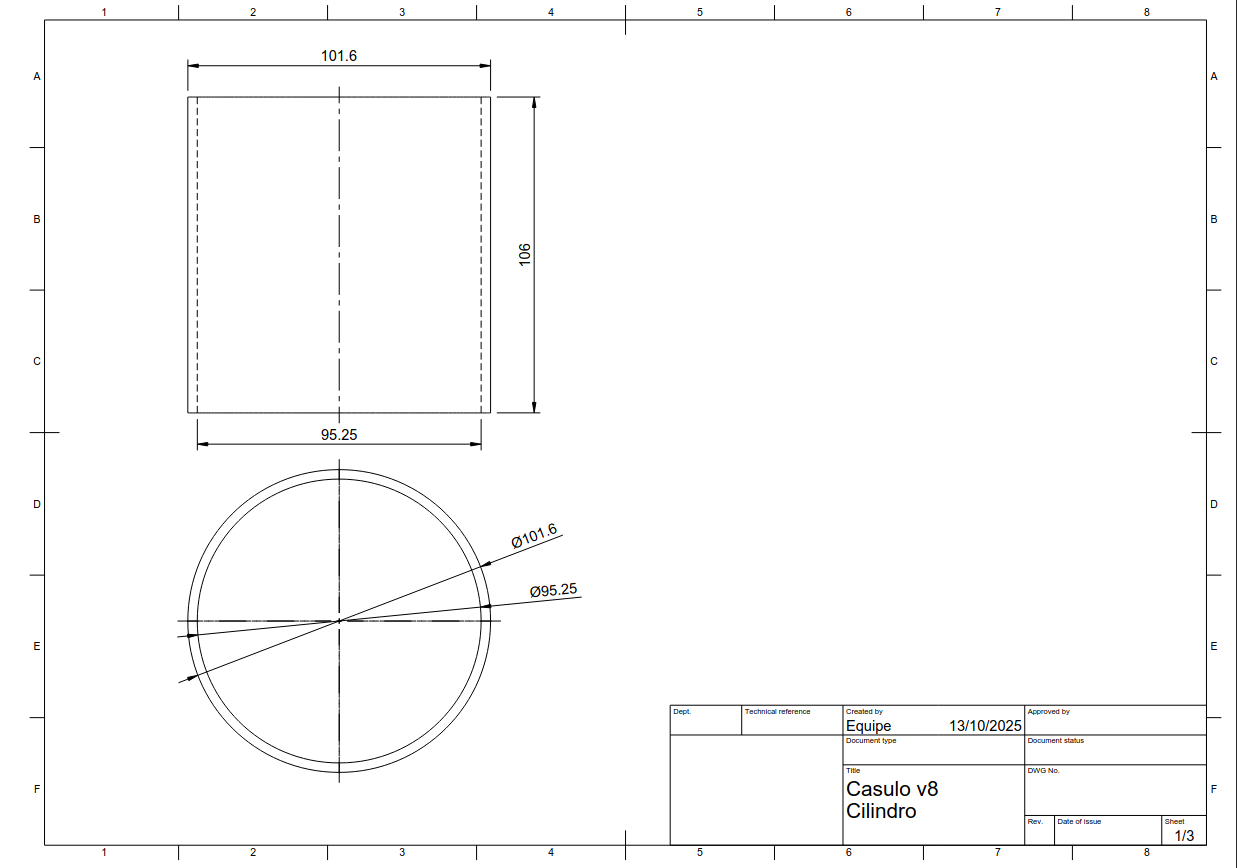
\includegraphics[width=.95\linewidth]{imagens/Screenshot from 2025-10-13 08-56-57.png}
    
    \label{fig:enter-label}
    \textbf{Fonte: } Autor
\end{figure}

\newpage
\end{document}